% This is "sig-alternate.tex" V2.1 April 2013
% This file should be compiled with V2.5 of "sig-alternate.cls" May 2012
%
% This example file demonstrates the use of the 'sig-alternate.cls'
% V2.5 LaTeX2e document class file. It is for those submitting
% articles to ACM Conference Proceedings WHO DO NOT WISH TO
% STRICTLY ADHERE TO THE SIGS (PUBS-BOARD-ENDORSED) STYLE.
% The 'sig-alternate.cls' file will produce a similar-looking,
% albeit, 'tighter' paper resulting in, invariably, fewer pages.
%
% ----------------------------------------------------------------------------------------------------------------
% This .tex file (and associated .cls V2.5) produces:
%       1) The Permission Statement
%       2) The Conference (location) Info information
%       3) The Copyright Line with ACM data
%       4) NO page numbers
%
% as against the acm_proc_article-sp.cls file which
% DOES NOT produce 1) thru' 3) above.
%
% Using 'sig-alternate.cls' you have control, however, from within
% the source .tex file, over both the CopyrightYear
% (defaulted to 200X) and the ACM Copyright Data
% (defaulted to X-XXXXX-XX-X/XX/XX).
% e.g.
% \CopyrightYear{2007} will cause 2007 to appear in the copyright line.
% \crdata{0-12345-67-8/90/12} will cause 0-12345-67-8/90/12 to appear in the copyright line.
%
% ---------------------------------------------------------------------------------------------------------------
% This .tex source is an example which *does* use
% the .bib file (from which the .bbl file % is produced).
% REMEMBER HOWEVER: After having produced the .bbl file,
% and prior to final submission, you *NEED* to 'insert'
% your .bbl file into your source .tex file so as to provide
% ONE 'self-contained' source file.
%
% ================= IF YOU HAVE QUESTIONS =======================
% Questions regarding the SIGS styles, SIGS policies and
% procedures, Conferences etc. should be sent to
% Adrienne Griscti (griscti@acm.org)
%
% Technical questions _only_ to
% Gerald Murray (murray@hq.acm.org)
% ===============================================================
%
% For tracking purposes - this is V2.0 - May 2012


\documentclass{sig-alternate-05-2015}

\usepackage{algorithm}
\usepackage{algorithmic}

\begin{document}

% Copyright
\setcopyright{acmcopyright}
%\setcopyright{acmlicensed}
%\setcopyright{rightsretained}
%\setcopyright{usgov}
%\setcopyright{usgovmixed}
%\setcopyright{cagov}
%\setcopyright{cagovmixed}


% DOI
\doi{10.475/123_4}

% ISBN
\isbn{123-4567-24-567/08/06}

%Conference
\conferenceinfo{PLDI '13}{June 16--19, 2013, Seattle, WA, USA}

\acmPrice{\$15.00}

%
% --- Author Metadata here ---
\conferenceinfo{WOODSTOCK}{'97 El Paso, Texas USA}
%\CopyrightYear{2007} % Allows default copyright year (20XX) to be over-ridden - IF NEED BE.
%\crdata{0-12345-67-8/90/01}  % Allows default copyright data (0-89791-88-6/97/05) to be over-ridden - IF NEED BE.
% --- End of Author Metadata ---

\title{A Novel Failure Detection Solution with Multiple QoS in Data Center Networks }
%
% You need the command \numberofauthors to handle the 'placement
% and alignment' of the authors beneath the title.
%
% For aesthetic reasons, we recommend 'three authors at a time'
% i.e. three 'name/affiliation blocks' be placed beneath the title.
%
% NOTE: You are NOT restricted in how many 'rows' of
% "name/affiliations" may appear. We just ask that you restrict
% the number of 'columns' to three.
%
% Because of the available 'opening page real-estate'
% we ask you to refrain from putting more than six authors
% (two rows with three columns) beneath the article title.
% More than six makes the first-page appear very cluttered indeed.
%
% Use the \alignauthor commands to handle the names
% and affiliations for an 'aesthetic maximum' of six authors.
% Add names, affiliations, addresses for
% the seventh etc. author(s) as the argument for the
% \additionalauthors command.
% These 'additional authors' will be output/set for you
% without further effort on your part as the last section in
% the body of your article BEFORE References or any Appendices.

%\numberofauthors{8} %  in this sample file, there are a *total*
% of EIGHT authors. SIX appear on the 'first-page' (for formatting
% reasons) and the remaining two appear in the \additionalauthors section.
%
\numberofauthors{2}
\author{
% You can go ahead and credit any number of authors here,
% e.g. one 'row of three' or two rows (consisting of one row of three
% and a second row of one, two or three).
%
% The command \alignauthor (no curly braces needed) should
% precede each author name, affiliation/snail-mail address and
% e-mail address. Additionally, tag each line of
% affiliation/address with \affaddr, and tag the
% e-mail address with \email.
%
% 1st. author
\alignauthor
Kai Shen\\
       \affaddr{School of Software}\\
       \affaddr{Shanghai Jiao Tong University}\\
       \affaddr{Shanghai, China}\\
       \email{knshen@sjtu.edu.cn}
% 2nd. author
\alignauthor
????\\
       \affaddr{????}\\
       \affaddr{Shanghai Jiao Tong University}\\
       \affaddr{Shanghai, China}\\
       \email{????@sjtu.edu.cn}
}

\maketitle

\begin{abstract}
Large scale data center networks are complex due to hundreds of thousands devices and links in them. Failures of these devices and links sometimes can lead to user-perceived service interruptions. Thus automated failure detection plays a very important role in maintaining the reliability of data centers. Many researches have been performed on failure detection in networks or distributed systems, but few of them identifies quality of service (QoS) multiplicity of failure detection in data center networks.

In this paper, to tackle with this problem, we firstly divide network devices into two categories: imperative devices whose failures need to be detected in real time, and non-imperative devices. Subsequently, we leverage a co-detection approach named K-detectors to detect failures of imperative devices, while the key idea of non-imperative devices failure detection is to analyze network traffic changes over time.

We evaluate our approach on a simulated network built by ns-3. Experimental results show that for imperative devices, our approach has a better QoS except for limited detection time increase in the presence of normal message loss and different size of failures. For non-imperative devices, our approach outperform existing work in terms of accuracy and failure discrimination.
\end{abstract}


%
% The code below should be generated by the tool at
% http://dl.acm.org/ccs.cfm
% Please copy and paste the code instead of the example below.
%
\begin{CCSXML}
<ccs2012>
 <concept>
  <concept_id>10010520.10010553.10010562</concept_id>
  <concept_desc>Computer systems organization~Embedded systems</concept_desc>
  <concept_significance>500</concept_significance>
 </concept>
 <concept>
  <concept_id>10010520.10010575.10010755</concept_id>
  <concept_desc>Computer systems organization~Redundancy</concept_desc>
  <concept_significance>300</concept_significance>
 </concept>
 <concept>
  <concept_id>10010520.10010553.10010554</concept_id>
  <concept_desc>Computer systems organization~Robotics</concept_desc>
  <concept_significance>100</concept_significance>
 </concept>
 <concept>
  <concept_id>10003033.10003083.10003095</concept_id>
  <concept_desc>Networks~Network reliability</concept_desc>
  <concept_significance>100</concept_significance>
 </concept>
</ccs2012>
\end{CCSXML}

\ccsdesc[500]{Computer systems organization~Embedded systems}
\ccsdesc[300]{Computer systems organization~Redundancy}
\ccsdesc{Computer systems organization~Robotics}
\ccsdesc[100]{Networks~Network reliability}


%
% End generated code
%

%
%  Use this command to print the description
%
%\printccsdesc

% We no longer use \terms command
%\terms{Theory}

\keywords{Failure detection; Quality of Service; Data center networks}

\section{Introduction}
Data center is a pool of resources interconnected using a communication network, a broad range of services (e.g., Web search, data analytic, storage backup) are hosted on data centers. Data center networks play a pivotal role in data centers as they integrate various resources and connect hundreds of thousands devices together (e.g. routers, switches, servers). For example, the Microsoft Live online services are supported by a Chicago-based
data center spanning more than 700,000 square feet \cite{DBLP:series/sbcs/LiuMVLH13}.

Due to the complexity and scale of data center networks, failures are common. Hence it is crucial to detect failures in the networks efficiently and effectively. Traditionally, domain experts are responsible for failure detection with the help of network monitoring data. But such a manual process is time-consuming, error-prone and not scalable. So automated failure detection approaches are useful in terms of helping reduce mean-time-to-recovery and service disruption.

However, failure detection in data center networks should not be simplex. On one hand, data center networks are reliable due to the built-in redundancy of data center networks like hardware redundancy and fault-tolerant routing protocols. Evidence shows that for about 80\% of the links and about 60\% of the devices, there is a more than four 9's of availability \cite{gill2011understanding}. On the other hand, many applications hosted on data centers have very strict timing constraints \cite{tomsic20152w}, they require failure detectors to provide quality of service (QoS) with quantitative timeliness guarantees.

Unfortunately, few researches have noticed QoS difference in failure detection of data center networks. Some researches on failure detection architecture such as \cite{felber1999failure}\cite{van1998gossip}\cite{gillen2007scalable}\cite{xu2012smart}\cite{xu2012smart} focus on the scalability issue of process crash detection in large scale distributed systems without considering underlying network topologies, while other work on failure localization in data center networks such as \cite{bahl2007towards}\cite{herodotou2014scalable}\cite{kandula2005shrink} treat all the network devices equally and utilize a general detection approach.

To address this issue, we firstly divide network devices into two categories: imperative devices and non-imperative devices. Imperative devices mainly include servers, top of rack switches and links between them, while non-imperative devices include other routers, switches and links. The main difference between them is that imperative devices have strict timing constraints of QoS as the failures of them may affect application functionalities. Naturally, our detection approach is two-fold: for imperative devices, we propose a co-detection model called K-detectors model to ensure the timeliness, soundness and accuracy at the same time. For non-imperative devices, we utilize a data mining based model to produce a ranked list consisting of suspect devices by extracting network traffic features. To evaluate our work, we compare our approach with hierarchical detection architecture \cite{felber1999failure} in terms of detection for imperative devices, and the work of Herodotou et al. \cite{herodotou2014scalable} in terms of detection for non-imperative devices. The experimental results prove the effectiveness of our work.

This paper makes the following contributions:
\begin{itemize}
  \item We identify the differences in QoS of failure detection in data center networks.
  \item We further divide network devices into two categories and propose effective failure detection approaches for these two kinds of devices respectively.
  \item We set up a series of evaluation metrics to evaluate different aspects of failure detection approaches.
  \item We implement our approach as well as other baselines on the same simulated data center network and prove the effectiveness of our approach.
\end{itemize}

The rest of the paper is organized as follows. Section 2 discusses related work. Section 3 presents data center networks architecture. Section 4 provides an overview of our approach, while the details are described in Section 5. The experimental evaluation along with experimental results is presented in Section 6. Finally, Section 7 concludes this paper.

\section{Related Work}
In this section, we will present various relevant works including failure detectors, failure detection architecture in distributed systems and failure detection in networks.

\subsection{Failure Detectors}
A failure detector (FD) is widely recognized as an oracle to intelligently suspect failed processes \cite{chandra1996unreliable}. The monitored process periodically send heartbeat messages to its detector to prove its liveness.

Chen et al. proposed a FD that provides QoS \cite{chen2002quality}. It estimates the expected arrival time (EAs) of the next heartbeat message according to a slide window storing $n$ most recent arrived messages. EAs determine the deadline that the detector will wait for the next heartbeat before suspecting the monitored process. \textit{Chen FD} can adjust current network condition and set the timeout threshold adaptively by referring to recent heartbeats. Bertier et al. proposed a similar FD \cite{bertier2002implementation}, whereas it uses a dynamic way to compute error margin of \textit{Chen FD}. Other FDs like \textit{$\phi$ Accrual FD} \cite{hayashibara2004varphi} and \textit{Satzger FD} \cite{satzger2007new} can output a continuous accrual failure value rather than a binary value which stands for the failure probability of the process at any time.

\subsection{Failure Detection Architecture}
A failure detection architecture aims to provide the service of monitoring nodes in large scale distributed systems in a scalable way.
Roughly speaking, there are two kinds of architectures. The first one is hierarchical architecture \cite{felber1999failure}, all the nodes are partitioned into different groups, each group has a leader node. Within a group, the leader node is responsible for monitoring all the other nodes. Leader nodes periodically send node status information of his group to other leader nodes. Hierarchical architecture can reduce the number of heartbeat messages effectively, but it exists \textit{Single Point of Failure} problem, when the leader node crashes, it needs to select a new leader.

Another alternative solution is Gossip-Style architecture \cite{van1998gossip}. Each node maintains a list containing the \textit{heartbeat counter} for each node in the system. Every T$_{gossip}$ seconds, each node firstly update \textit{heartbeat counter} of itself and then randomly select another node to send its list to. Upon receiving a message, the node will merge two lists and update each node's \textit{heartbeat counter} with the bigger one. If the \textit{heartbeat counter} does not update after T$_{fail}$ seconds, the node will be marked as crashed. If the \textit{heartbeat counter} does not update after T$_{cleanup}$ (T$_{cleanup}$
$\ge$T$_{fail}$) seconds, it will be removed from the list. This approach has very low bandwidth occupation because it only produces $n$ messages each epoch where $n$ is the size of the system. However, with the increasing of crashing nodes, it needs more time to detect these failures.

\subsection{Failure Detection in Networks}
Different from the work mentioned above, failure detection in networks take network topology into consideration and localize failure positions at IP layer. Gill et al. present the first large-scale survey on failures in data center networks \cite{gill2011understanding}.

Also, there exists a large body of work on applying statistical approaches to failure localization in networks. \textit{Sherlock} \cite{bahl2007towards} localizes failures to limited network components by capturing dependencies between components. \textit{Shrink} \cite{kandula2005shrink} leverages Bayesian Network model to diagnose root cause of IP network failures. Herodotou et al. \cite{herodotou2014scalable} actively inject ping traffic into network and analyze the ping results overlaid on top of the network topology, it generates a ranked list containing the suspected failed device and links along with their failure score that can best explain the observed ping data.

% figure
\begin{figure}[t]
\centering
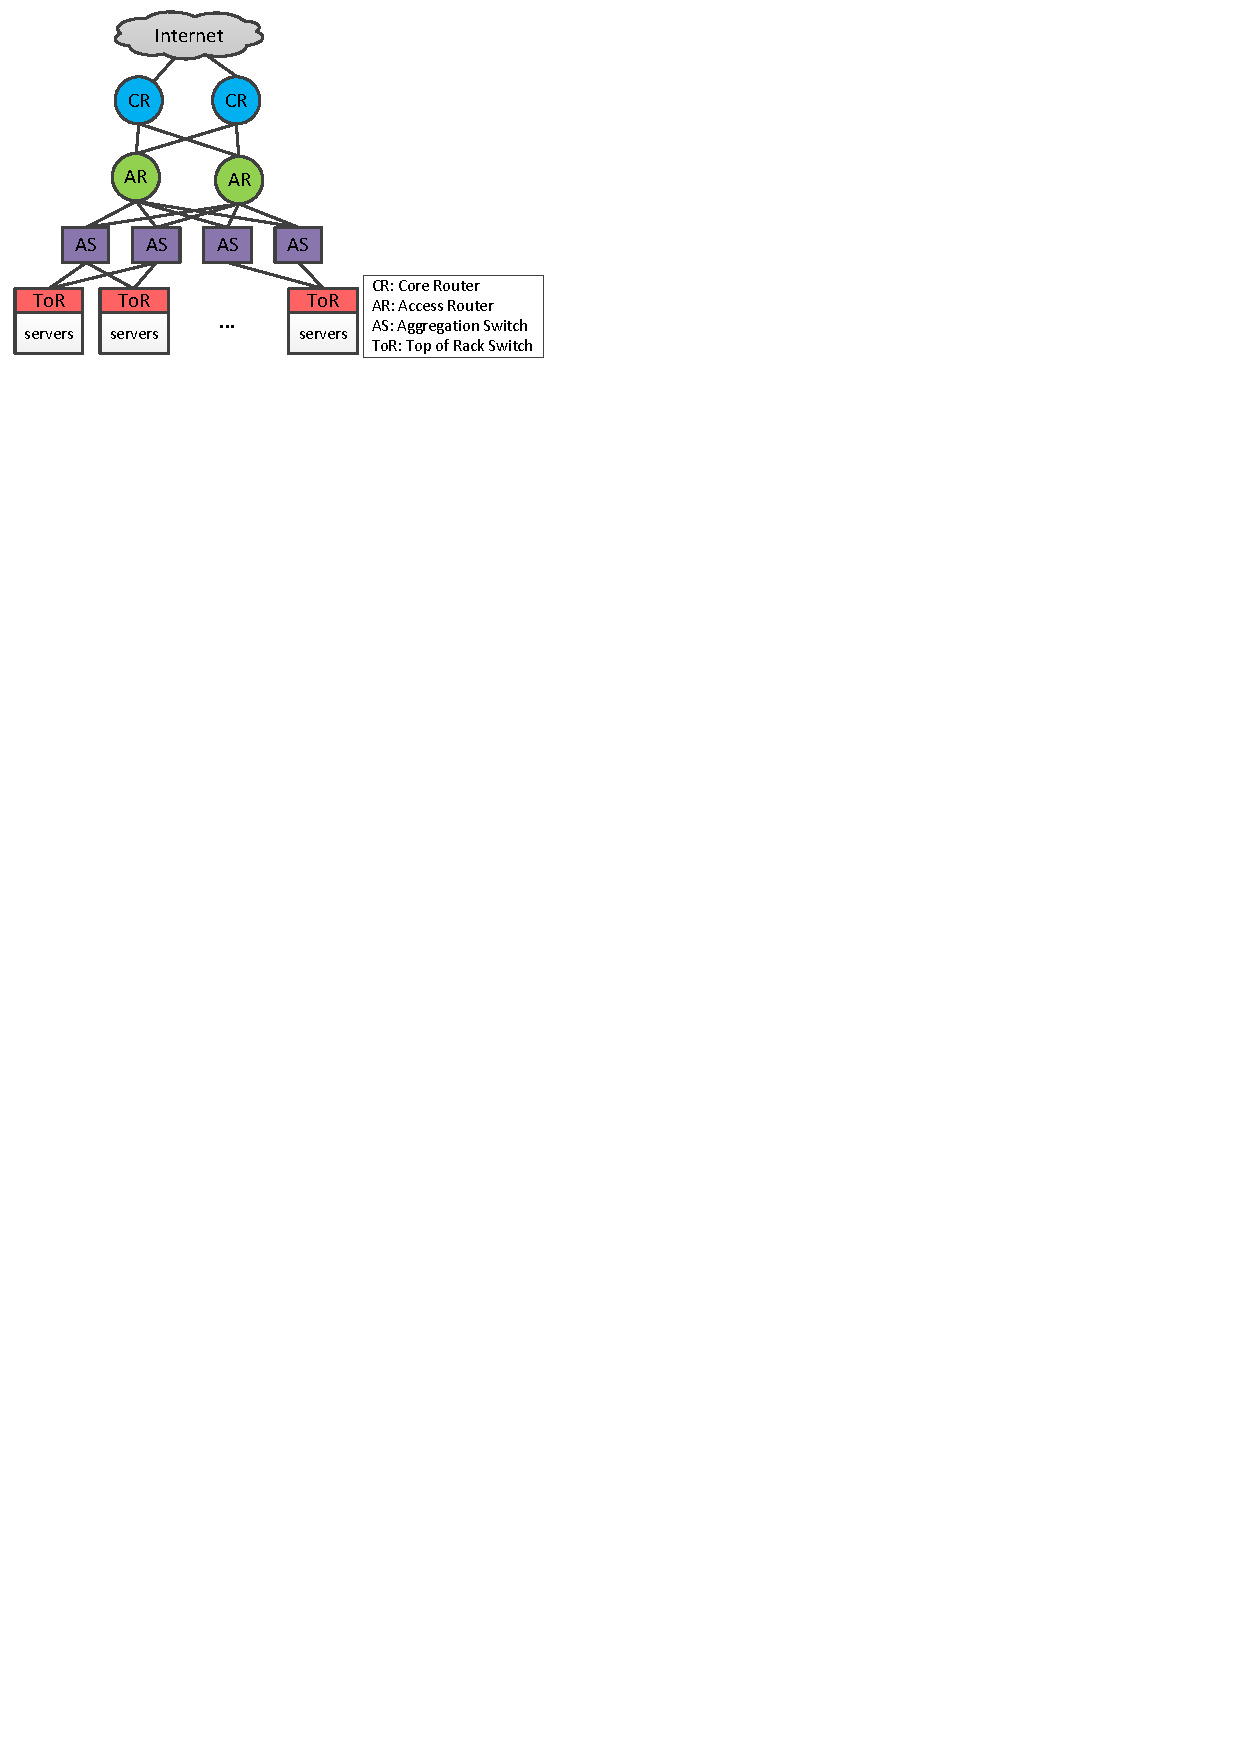
\includegraphics{topology}
\caption{Conventional Data Center Network Topology}
\end{figure}

\section{Data Center Network Architecture}
In this section, we will take a brief look at common data center network architecture.

A data center is a facility used to house computer systems and associated components, it usually contains hundreds of thousands devices and links. Modern data centers use hierarchical architectures. Figure 1 depicts a conventional data center network architecture \cite{gill2011understanding}\cite{greenberg2009vl2}\cite{herodotou2014scalable}. At the bottom layer are racks of servers, typically there are 20 to 40 servers in each rack, and each server in the same rack connects to a Top of Rack (ToR) Switch via a 1 Gbps link. Each ToR then connects to a primary and a backup Aggregation Switch (AS) for redundancy. ASs are connected to Access Routers (ARs) forming a complete bipartite graph. Finally, ARs are connected to Core Routers (CRs). CRs are at the boundary of a data center network.

To limit overheads and also to isolate different services, servers are partitioned into virtual LANs (VLANs). All links in the data center use Ethernet as link layer protocol and physical connections are a mix of copper and fiber cables. In addition to the devices in Figure 1, there may exist other devices like Load Balancers (LBs) and Firewalls.

Modern data center usually employs \textit{Equal Cost MultiPath (ECMP)} routing within the data center for fault tolerance, which means that given a source and destination, there are multiple paths from the source to the destination. Thus in this work, we will apply ECMP routing to the simulated network by enabling ECMP routing configurations in ns-3.


\section{Approach Overview}
In this section, we will introduce the whole design of our failure detection approach.

As we mentioned in Section 1, different network device should have different quality of service (QoS). Gill et al. \cite{gill2011understanding} have shown the diversity of different devices' failure characteristics. Unfortunately, none of the work in Section 2 treats these devices differently. We firstly divide network devices into two categories.

\begin{itemize}
\item \textbf{Imperative Device.} This category includes servers, ToRs and links between ToRs and servers. Typically servers run various user applications and store user data. The crash of servers may cause user-perceived faults. The crash of a ToR will make servers under it unreachable. Also Gill et al. declare that the downtime of ToRs may be very long. Thus the failure detection for these devices must be fast enough besides other requirements.

\item \textbf{Non-imperative Device.} It includes links, other routers and switches. A single failure of a link or a router does not affect the functionality of a data center because of built-in redundancy in data centers. So the data center administrators care more about whether the detection service is accurate enough to help them localize the real faults.

\end{itemize}

% figure
\begin{figure}[t]
\centering
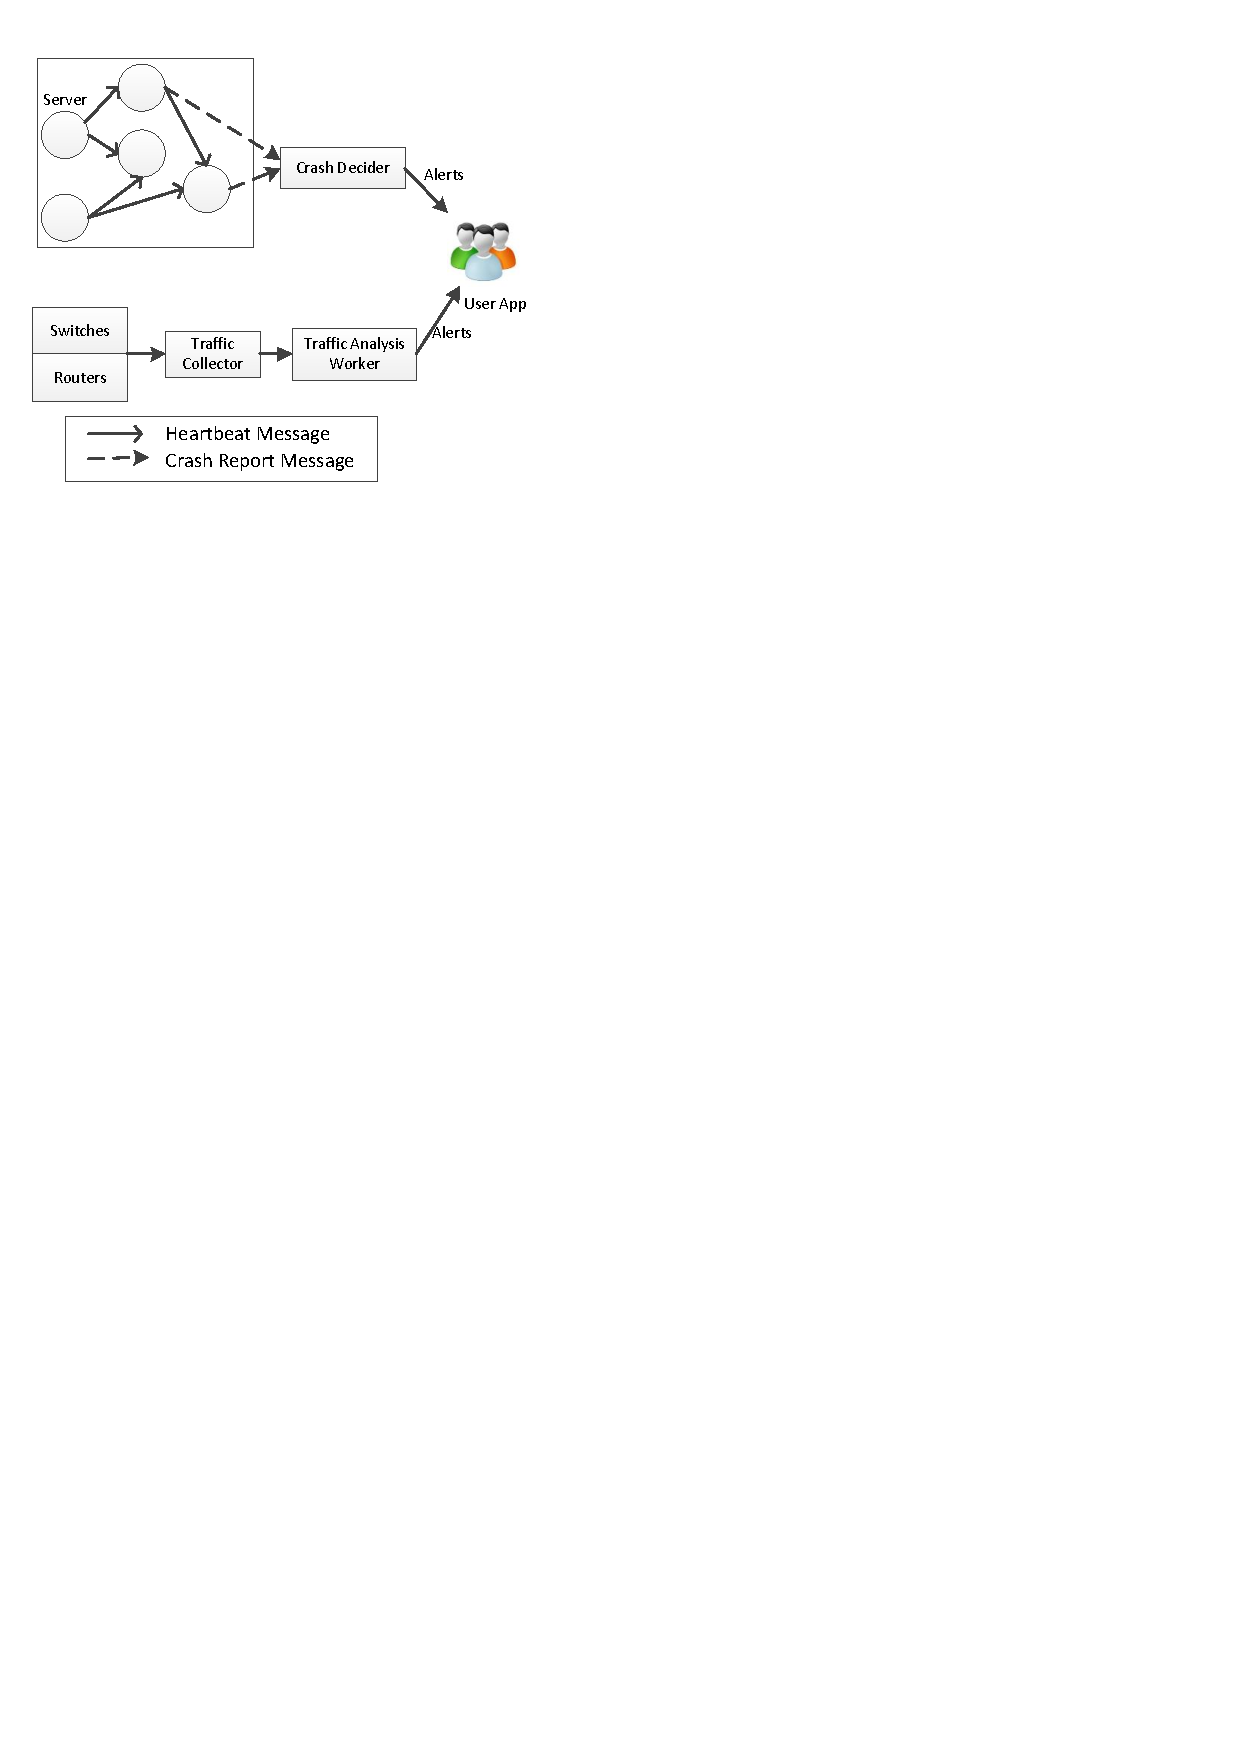
\includegraphics{system}
\caption{Failure Detection System Architecture}
\end{figure}

Figure 2 illustrates the entire architecture of our failure detection system. It mainly contains two modules. The upper half part illustrates the module for server failure detection. It is a combination of centralized and decentralized structures. A server can both play the role of a detector and a monitored object. Each server is monitored by multiple FD processes installed on different servers for redundancy. A server can also monitor a group of servers. Once a FD determines the crash of a server, it will send a crash report message to \textbf{Crash Decider}. \textbf{Crash Decider} will determine the final status of this server. On top of this, \textbf{Crash Decider} is also responsible for detecting ToR failures by combining all the server crash report messages together.

For the detection of non-imperetative devices, \textbf{Traffic Collector} periodically collects traffic data of routers and switches and send telemetry data to \textbf{Traffic Analysis Worker}. \textbf{Traffic Analysis Worker} finally generate failure alerts by performing analysis on these data.



\section{Failure Detection Approach}
In this section, we will discuss the detailed design of different aspects of the failure detection system respectively.

\subsection{K-detectors Model}
To detect the crash of servers and ToRs effectively and efficiently, this paper propose a co-detection model named $K$-detectors model. Our detection model is based on the assumption that once the server or ToR crashes, it never recovers by itself. We first refine the QoS of failure detection for servers:

\begin{itemize}
\item \textbf{Efficiency.} It measures how fast the system can report the crash after it crashes. The system is more efficient if it takes less time to detect a failure. In particular, server failures should be detected in real time.
\item \textbf{Completeness.} It measures whether the system can detect all the crashed objects. The system is more complete if it rules out fewer true crashed ones.
\item \textbf{Soundness.} In some scenarios, the behavior of the network may vary. For example, message loss and message delay may happen sometimes. The detection system should be sound enough to distinguish between such conditions and a real crash.

\end{itemize}

In $K$-detectors model, each server is monitored by $K$ FDs on different servers where $K$ is a parameter tuned by user applications. When a FD considers a server crashes, it sends a crash report message to \textbf{Crash Decider}. If the output of the FD transforms from suspect to trust, it re-sends a message to revoke the most recent crash report.

\begin{equation}
S_{s,t}=\left\{
    \begin{array}{lcl}
    \text{suspect} & \text{if} & |\,CRM_{s,t}\,|\geq\left\lfloor(K+1)/2\right\rfloor \\

    \text{trust} && \text{otherwise}
    \end{array}
\right.
\end{equation}
where $CRM_{s,t}$ denotes the collection of crash report messages for server $s$ until time $t$, $S_{s,t}$ denotes the status of server $s$ at time $t$. If \textbf{Crash Decider} receives $\left\lfloor(K+1)/2\right\rfloor$ crash messages of a server, it considers the server to have crashed. So a server is still under monitor even when a number of its FDs crash.

\subsection{Monitoring Rule Inference}
A monitoring rule defines the monitoring relationships among a group of servers. To form the $K$-detectors model and also to meet QoS to the greatest extent, we propose the following specifications of a monitoring rule:
\begin{enumerate}
    \item Each sever monitors $K$ servers. This balances monitor intensity of each server.
    \item A server cannot monitor itself.
    \item A server is monitored by $K$ different servers.
    \item $K-1$ of the $K$ detectors are on the servers at the same rack.
    \item The monitoring rule should ensure each link covered by heartbeat messages.
    \item Each rack monitors servers of other racks which vary from different racks averagely.
\end{enumerate}

\subsubsection*{Rationale}
\quad Intuitively, the use of $K$ FDs is able to adapt to bursty-traffic conditions like message loss because the determination of a failure requires at least $\left\lfloor(K+1)/2\right\rfloor$ FDs' agreement. Also, $K$-detectors can prevent crashes of FDs to some extent. Theoretically, a failure can still be detected even when $K-\left\lfloor(K+1)/2\right\rfloor=\left\lfloor K/2\right\rfloor$ of its detectors crash.

On the other hand, the fourth specification above can make the best of locality of LAN, which reduces the probability of degeneration on detection time in turn.

Specification five is the presupposition of link failure detection. It is easy to see that, some links cannot be distinguished from faulty links without this specification.

The last one is an extension of specification five. It is for the consideration of ToRs' failure detection, we will discuss it in detail in Section 5.4.

\subsection{FD Algorithm}
FD algorithm is used to decide the status of one monitored object by one FD. Our FD algorithm is almost the same as \textit{Chen FD} \cite{chen2002quality} except for some minor changes.

\begin{equation}
EA_{l+1} \approx \frac{1}{n}(\sum_{i=1}^{n}A_i - \eta s_i)+(l+1)\eta
\end{equation}
this formula estimates the expected arriving time of next message, where $s_i$ is the sequence number of heartbeat message, $A_i$ is the receipt time of message $i$, $\eta$ is message send interval. Obviously, this formula normalizes each $A_i$ by shifting it backward $\eta s_i$ time units.

After that, we utilize Hyperbolic Tangent Function to model current suspicious level:

\begin{equation}
\tau(t_{now}) = |\,tanh(t_{now}-EA_{l+1})\,|
\end{equation}
Hyperbolic Tangent Function is one of the widely used activation functions in neural networks. The suspicious level $\tau(t_{now})$ always ranges from 0 to 1, when $t_{now}$ grows bigger, the suspicious level is closer to 1, which implies a higher failure probability. A continuous valued rather than binary valued output decouples the interpretation of failure data from the failure monitoring mechanism, user applications can set their own threshold according to their demands.

\subsection{Failure Detection for ToRs}
Apart from determination of servers' crashes, \textbf{Crash Decider} is also responsible for failure detection for ToRs. The essential idea is that if most or even all servers in a rack is reported crash by FDs in other racks, it is more likely that the top of rack switch crashes rather than the servers.

\begin{equation}
S_{ToR,t}=\left\{
    \begin{array}{lcl}
    \text{suspect} & \text{if} & |\, \{s\, |\, s \in ToR, \\
    && CRMO_{s,t} \not = \emptyset, \\
    && |\,CRM_{s,t}\,|=1\} \,| \geq \alpha \cdot m \\

    \text{trust} && \text{otherwise}
    \end{array}
\right.
\end{equation}
where $m$ is the number of servers per rack, $\alpha$ is a  proportionality coefficient measuring how strict the criterion is to determine failure of a ToR. $CRMO_{s,t}$ denotes the collection of crash report messages of $s$ coming from outside racks until time $t$. When \textbf{Crash Decider} gets more than $\alpha \cdot m$ crash report messages of servers under the ToR crash, it will report the crash of ToR. The last specification in Section 5.2 ensures that once a ToR is down, each other rack has the chance to find this failure. Suppose there are $n$ racks in total, according to this specification, for each rack $r$, each other rack will monitor $m/(n-1)$ servers of rack $r$. An extreme counter-example is that if the outside detectors of rack 1 servers are all in rack 2, once ToR of rack 2 is down, \textbf{Crash Decider} never perceives the status of ToR of rack 1.

\subsubsection*{Upper Bound of $\alpha$}
Theoretically, a smaller $\alpha$ means a more aggressive detection. We can set an appropriate $\alpha$ empirically by looking back on historical data on ToR crashes. Suppose we have known the ToR crash probability $p$, there are $n$ racks (each one has a ToR) and crashes of ToRs are subject to \textit{binomial distribution}. When there are $k$ ToR crashes, the number of server crash report messages we can observe $m^\prime$ should be
\begin{equation}
    m^\prime  = \frac{m}{n-1}(n-k) = \frac{m(n-k)}{n-1}
\end{equation}
Thus the value of $\alpha$ is at most:
\begin{equation}
    \alpha  = \frac{m^\prime}{m} = \frac{n-k}{n-1}
\end{equation}
Next, if given a confidence parameter $p_0$,
\begin{equation}
    \begin{aligned}
        &\alpha \leq \alpha_0  = \frac{m_0^\prime}{m} = \frac{n-k_0}{n-1}\\
        &\text{where } k_0 \text{ is the minimum of } k\\
        & s.t. \quad Pr(x\leq k) = \sum_{r=0}^k C_n^r p^r(1-p)^{n-r} \geq p_0 \\
    \end{aligned}
\end{equation}
$Pr(x\leq k)$ denotes the probability of number of ToR crashes is no more than $k$. Hence the theoretical upper bound of $\alpha$ is $\alpha_0$. Actually, because of server crashes, the number of crash report messages \textbf{Crash Decider} can receive may less than observe $m_0^\prime$, so the value of $\alpha$ should be less than its upper bound.

To sum up, Algorithm 1 illustrates the pseudo-code for overall detection algorithm of \textbf{Crash Decider}.
\renewcommand{\algorithmicrequire}{\textbf{Input:}}
\renewcommand{\algorithmicensure}{\textbf{Output:}}
\begin{algorithm}
	\caption{Detection Algorithm of \textbf{Crash Decider}}
	%\label{alg0}
	\begin{algorithmic}[1]
		\REQUIRE $K$, $\eta$, $n$, $\alpha$, $m$, $\tau_m$
		\ENSURE $S_{i,t}$, $i \in \text{Imperative Device}$
	
        \FOR{$i \text{ in Imperative Devices}$}
            \STATE $S_{i,t_0} \leftarrow trust$
        \ENDFOR
	    \WHILE{$True$}
            \STATE $List<Integer> failsEachRack \leftarrow \emptyset$
            \FOR{each $i$ in Servers}
                \STATE $rackID \leftarrow getRackID(i)$
                \IF{$|\,CRM_{i,t_{now}}\,| \geq \left\lfloor(K+1)/2\right\rfloor$}
                    \STATE $S_{i,t_{now}} \leftarrow suspect$
                \ELSE
                    \STATE $S_{i,t_{now}} \leftarrow trust$
                    \IF{$\text{only one CRM coming from other rack}$}
                    \STATE $failsEachRack.get(rackID)\text{++}$
                    \ENDIF
                \ENDIF
            \ENDFOR

            \FOR{$\text{each } i \text{ in ToRs}$}
                \IF{$failsEachRack.get(i) \geq \alpha \cdot m$}
                    \STATE $S_{i,t_{now}} \leftarrow suspect$
                \ELSE
                    \STATE $S_{i,t_{now}} \leftarrow trust$
                \ENDIF
            \ENDFOR
		\ENDWHILE
	\end{algorithmic}
\end{algorithm}
It firstly determines the status of each server (line 6 to 16), and then determines the status of ToRs (line 17 to 23). When detecting server failures, \textbf{Crash Decider} also records necessary information to find potential ToR crashes (line 12 to 14).

\subsection{Failure Detection for Links}
The failure detection for non-imperative devices is another important part of our detection system. Failures of routers and switches can be easily detected by checking traffic dump on them. So in this subsection, we will focus on detection for links. We firstly refine the following QoS:
\begin{itemize}
  \item \textbf{Precision.} Precision indicates how many suspected links are true failed.
  \item \textbf{Completeness.} This measures whether our approach can find all the faulty links.
  \item \textbf{Discrimination.} Because we will provide a short ranked list of suspected objects, this measures to what degree can our approach distinguish between normal links and faulty links.
\end{itemize}

The key idea of our approach is to capture network traffic changes over time. If the network traffic changes significantly compared with traffic in normal conditions, we believe that there exists failures somewhere in the network. The insight is that network traffic distribution is associated with routing protocol and monitoring relationships of servers, the drastic changes of traffic probably imply failures. For example, if the network topology is just as Figure 1 shows, when the link between the leftmost AR and the leftmost AS fails, the heartbeat traffic on the leftmost AR will decrease and the rightmost AR's heartbeat traffic will increase according to \textit{ECMP} routing.

To collect required traffic data, we simply install \textit{tcpdump} on each router and switch. These data will be collected to \textbf{Traffic Analysis Worker} for further analysis.

In order to model this data analysis problem, this paper proposes a Back Propagation Neural Networks (BPNN) based method to compute failure probability of each link.

\subsubsection*{Feature Extraction}
\quad The first step is to extract rational features from raw traffic data. To address this issue, we extract $v \cdot n^2$ features in total. $v$ is number of devices (CRs, ARs, ASs), each device has $n^2$ features where $n$ is the number of racks. In particular, each feature denotes traffic of one direction. Obviously, there are $n$ choices of sources and $n$ choices of destinations, so the total number of possible traffic directions is $n^2$.
Formally, the traffic features during a time period $\Delta T$ is presented as \boldmath $x$
\unboldmath $=($\boldmath $x_1, x_2, ..., x_v$\unboldmath $)$, \boldmath $x_i$
\unboldmath $=(x_i^1, x_i^2, ..., x_i^{n^2})$
where $x_i^j$ stands for direction $j$ traffic of device $i$ in $\Delta T$.

\subsubsection*{BPNN Model}
\quad Suppose the number of links is $e$, for each time period $\Delta T$, the output of our model should be
\boldmath $y$
\unboldmath $=(y_1, y_2, ..., y_e)$, where $y_i$ denotes failure probability of link $i$. We apply a BPNN model to localize the faulty link during $\Delta T$. As is shown in Figure 3, BPNN is a multi-layer perceptron architecture:
\begin{figure}[t]
  \centering
  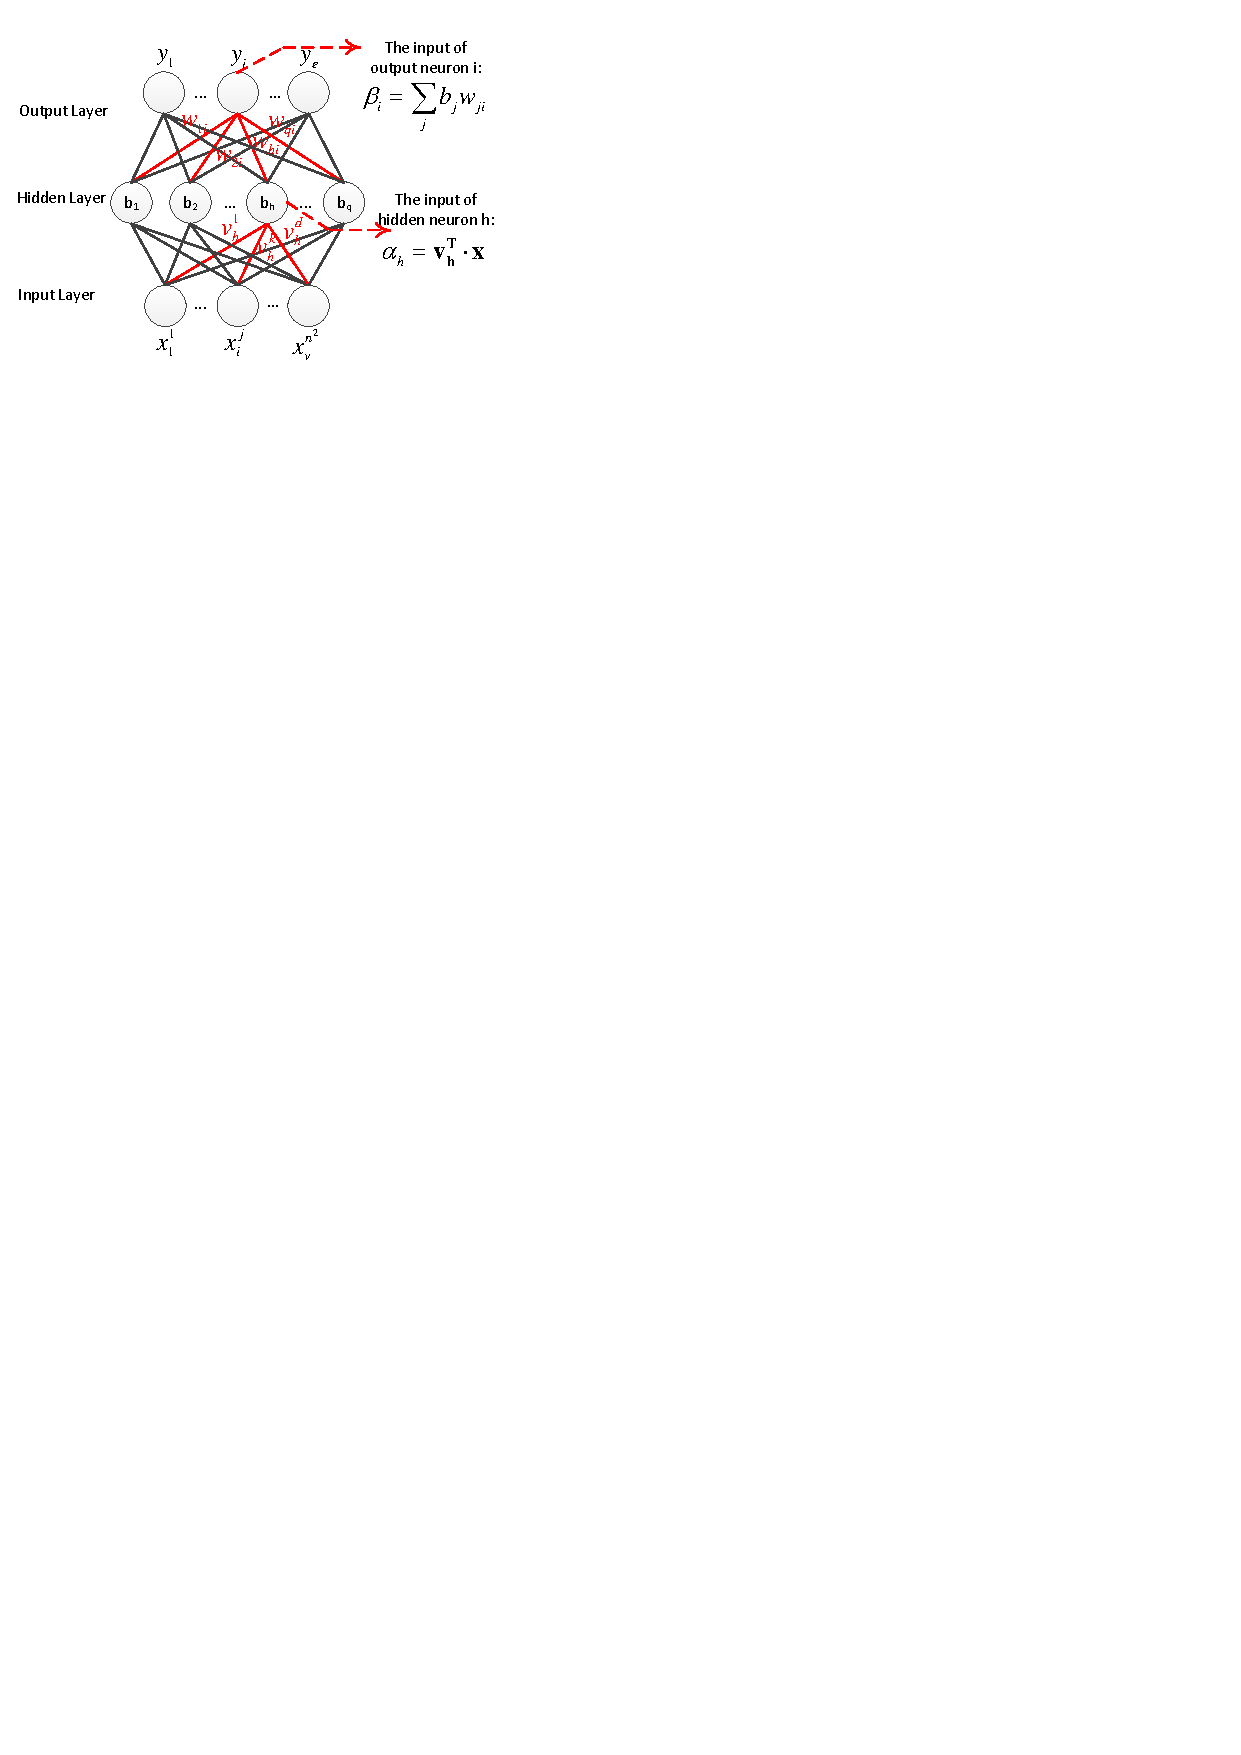
\includegraphics{ANN}
  \caption{Multi-layer Perceptron Architecture}
\end{figure}
To reduce the computational work of training, we only set one hidden layer, both the hidden layer neurons and output layer neurons utilize Sigmoid function as the activation function. Take the output layer as an example:
$y_i = Sigmoid(\beta_i - \theta_i)$ where $\theta_i$ is a constant term of the perceptron.

\subsubsection*{Training of BPNN}
\quad To train the neural network, we apply the classical error BackPropagation (BP) algorithm \cite{rumelhart1988learning}. BP algorithm is based on gradient descent strategy.% write BP algorithm?

To get train data, we manually disable links to simulate real link failures. To be specific, each time we disable one link for some time. After that, we collect dump data from each router and switch, extracting direction features just as mentioned above. The next step is to split the traffic data into different chunks, with each chunk representing the traffic data within one time unit ($\Delta T$). Each traffic chunk forms one train instance.

\subsubsection*{The Detection Algorithm}
\quad BPNN model is only able to identify the faulty link during one time unit, in the following part, we will introduce how we can detect multiple faults over time.

First of all, we assume that there are at most one link failure during a time unit ($\Delta T$). This assumption is partially supported by the finding proposed by Gill et al. They find that on an average, link failures tend to be separated by a period of about one week \cite{gill2011understanding}.

\renewcommand{\algorithmicrequire}{\textbf{Input:}}
\renewcommand{\algorithmicensure}{\textbf{Output:}}
\begin{algorithm}
	\caption{\textbf{Traffic Analysis Worker} Algorithm}
	\begin{algorithmic}[1]
        \REQUIRE \boldmath $x^t$ \unboldmath$=($\boldmath $x_1^t, x_2^t, ..., x_v^t$\unboldmath $)$
		\ENSURE $F_i \text{ for } i \in E$

        \STATE $\text{divide traffic data }$\boldmath $x^t$$\text{ into }$\unboldmath $\left\lfloor t/\Delta T \right\rfloor \text{ chunks}$

        \FOR{$i \in E$}
            \STATE $F_i \leftarrow 0$
        \ENDFOR
        \FOR{$\text{each data chunk } $ \boldmath $x$}
        \STATE \boldmath $y$\unboldmath $\leftarrow BPNN($\boldmath $x$\unboldmath $)$
            \FOR{$i \in E$}
                \STATE $F_i \leftarrow F_i + y_i$
            \ENDFOR
        \ENDFOR

        \FOR{\unboldmath $i \in E$}
            \STATE $F_i \leftarrow \frac{\Delta T \cdot F_i}{t}$
        \ENDFOR
        \STATE $\text{sort }$\boldmath $F$\unboldmath$\text{ in descending order}$
	\end{algorithmic}
\end{algorithm}

Algorithm 2 shows the algorithm of \textbf{Traffic Analysis Worker}. The input of the algorithm is the refined time series traffic data over time $t$. Firstly, traffic data is divided into chunks. Each chunk represents a time unit $\Delta T$ of traffic (line 1). The last chunk will be dropped if its time period is less than $\Delta T$. For each of traffic data chunk, we utilize the trained BPNN model to compute failure score of links during this time unit. The final failure score over $t$ is computed as the arithmetic mean of failure scores of all time units (line 5 to 13). This solution inevitably benefits the early happened faulty links. For example, when there are only one faulty links in the network, the failure score of the sole faulty link will be very high, which in turn makes its final failure score higher. However, it does not matter because we care more about whether it can find more failures rather than the ranking.


\section{Evaluation}
In this section, we will present how we evaluate our approach. Experimental results will also be shown in this section.

\subsection{Experimental Settings}
To build up a data center network, we deploy ns-3 on PC. ns-3 is a discrete-event network simulator for Internet systems, targeted primarily for research and educational use \cite{henderson2008network}. We install ns-3 on single PC with 2 cores, 3.4 GHz CPU and 4GB RAM. The version of ns-3 we use is ns-3.24.

We set up a simulated data center network following the topology in Figure 1. There are a total of 120 servers (20 servers $\times$ 6 racks), 14 routers and switches and 140 links. For each link, data rate is 100 Mbps, delay is 100 ms.

\subsection{Research Questions}
The objective of our experiments is to validate the effectiveness of the proposed approach compared with baselines. For this purpose, we set up the following research questions:

\subsubsection*{RQ1: Can K-detectors model benefit server failure detection?}
\quad RQ1 evaluates QoS of failure detection for servers. To answer this question, we firstly set four metrics \cite{chen2002quality} corresponding to the QoS in Section 5.1.
\begin{itemize}
  \item \textbf{Average Detection Time ($AT_D$)} is the average time that elapses from the crash of a server until the crash is reported.
  \begin{equation}
    AT_D = \frac{\sum_i(T_{D,i} - T_{C,i})}{n}
  \end{equation}
  where $n$ is the number of detected crashes, $T_{D,i}$ is the detection time of $i$th crash $i$, $T_{C,i}$ is the crash time of $i$th crash.

  \item \textbf{Average Mistake Rate ($AR_M$)} measures the average rate at which a FD suspects a correct object. It equals the number of such mistakes per unit of time. For example, suppose Figure 4 depicts the monitoring of the object in one time unit, the mistake rate of this FD is two.
\begin{figure}[t]
  \centering
  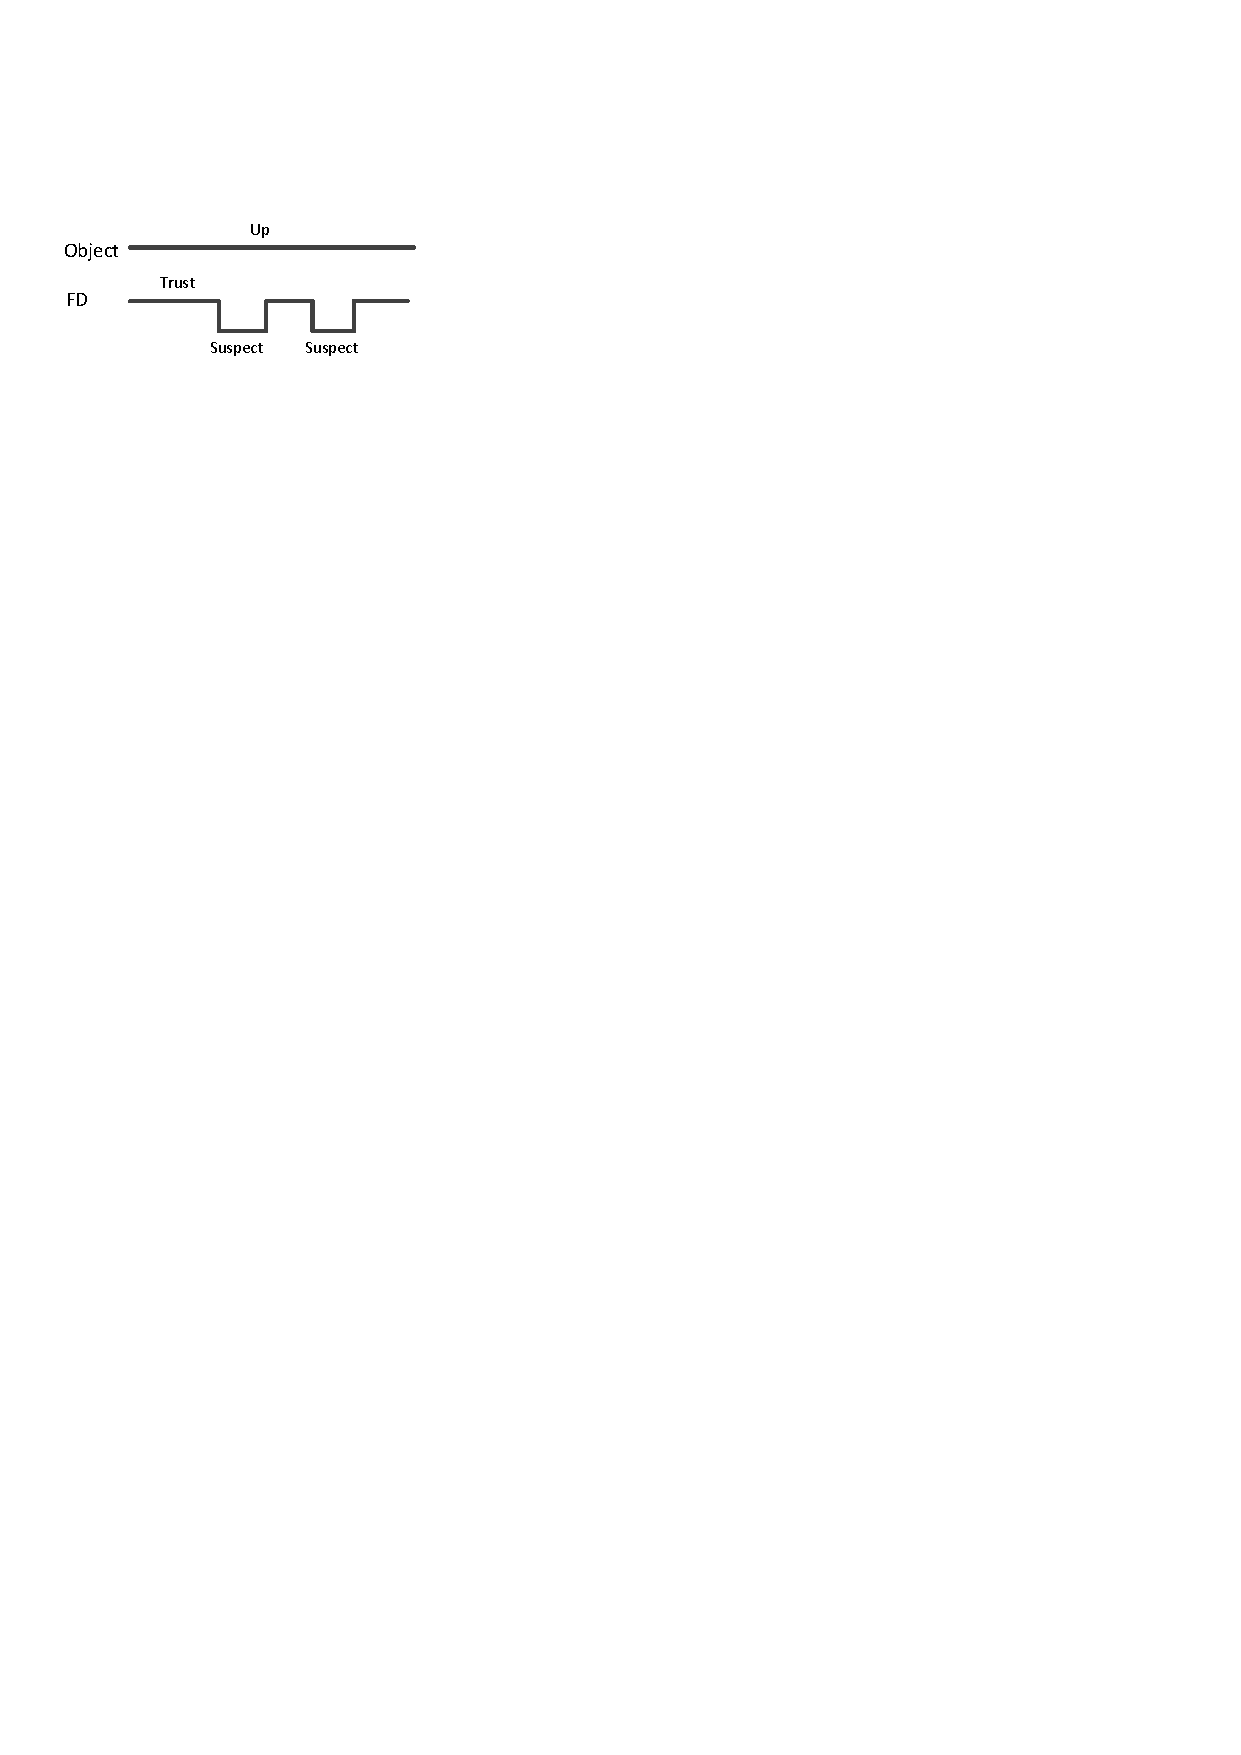
\includegraphics{metric}
  \caption{Average Mistake Rate}
\end{figure}

  \item \textbf{Query Accuracy Probability ($P_A$)} is the probability that the detection system outputs the correct results when queried at a random time.

  \item \textbf{Number of Undetected Crashes} measures the number of ignored real crash servers. This metric measures the completeness of the approach.
\end{itemize}

We compare our work with the traditional hierarchical architecture \cite{felber1999failure} in terms of the metrics above.

\subsubsection*{RQ2: Can K-detectors model benefit ToR failure detection?}
\quad The evaluation of failure detection for ToRs is similar to servers. We will evaluate the impact of different number of server crashes, that is to say, we want to see whether server failures affect the QoS of ToR failure detection. The evaluation metrics are the same as servers.

\subsubsection*{RQ3: Is the BPNN based approach effective?}
\quad This RQ evaluates whether the proposed approach is more effective in detecting link failures than existing work. We make another three metrics:
\begin{itemize}
    \item \textbf{Precision@k.} We make the use of this metric in order to evaluate to what degree the detection is accurate. This metric is appropriate because it does not take into account the positions in the list which caters to our requirements \cite{mogotsi2010christopher}.
    \begin{equation}
        precision@k = \frac{1}{n}\sum_{i=1}^n \frac{fail_{i,k}}{k}
    \end{equation}
    where $fail_{i,k}$ denotes the number of true failures for failure event $i$ in the top $k$ returned results. $n$ is the number of failure events, $k$ equals to the number of true failures. A perfect result is all the $k$ failures are ranked at the top $k$ positions.

    \item \textbf{MRR.} We also make use of Mean Reciprocal Rank (MRR), which is a statistic measure for evaluating a process that produces a ranked list to a sample of queries, the list contains items ordered by probabilities \cite{radev2002evaluating}. It is the average multiplicative inverse of the rank of the first faulty link:
        \begin{equation}
            MRR = \frac{1}{n}\sum_{i=1}^n \frac{1}{rank_i}
        \end{equation}

    \item \textbf{Discriminative Significance} (DS). DS is based on the notion of entropy. Entropy is a measure of unpredictability of information content \cite{shannon2001mathematical}.
        \begin{equation}
            DS = -\sum_{i=1}^e F_i \cdot log_2 F_i
        \end{equation}
        where $F_i$ is a normalized failure score of link $i$. We leverage this metric to evaluate discrimination of different detection approaches. A smaller DS implies that the results of ranked list is more determinate, which makes it easier for further troubleshooting.


\end{itemize}

We will compare this part of our approach with the work of Herodotou et al. \cite{herodotou2014scalable}.

\subsection{Experimental Results}

\subsubsection*{RQ1: Server failure detection}
\quad We evaluate our approach in the presence of different degrees of message loss and server crashes. To be fair, FD parameters of all the methods are set to the same: $\tau_m=0.001$, slide window size $n=100$. Heartbeat message send interval $\eta$ is 100 ms. The whole application is run for 1 min.

\begin{figure}[t]
  \centering
  \begin{tabular}{c}
  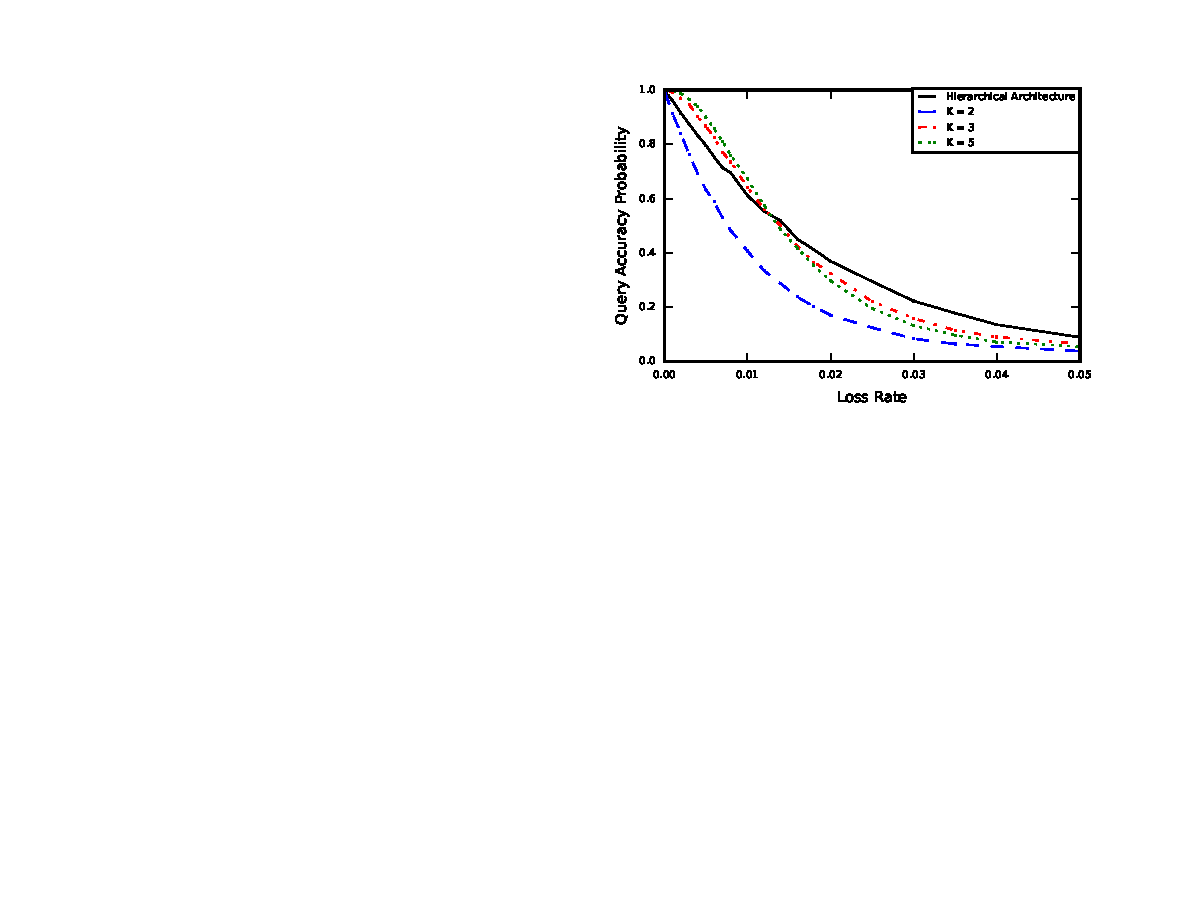
\includegraphics[scale=0.7]{r1} \\
  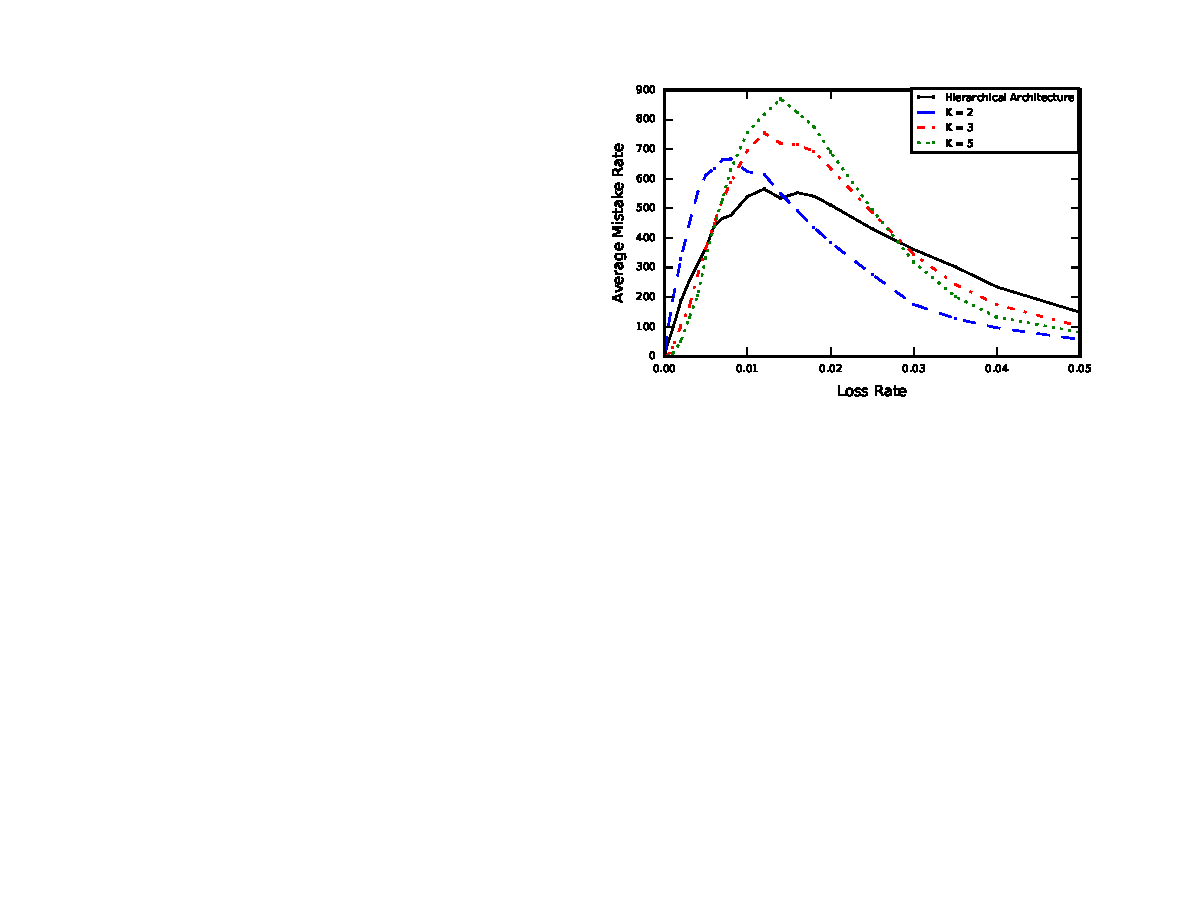
\includegraphics[scale=0.7]{r2}
  \end{tabular}
  \caption{Effect of Message Loss on $P_A$ and $AM_R$}
\end{figure}

\begin{figure}[t]
  \centering
  \begin{tabular}{c}
  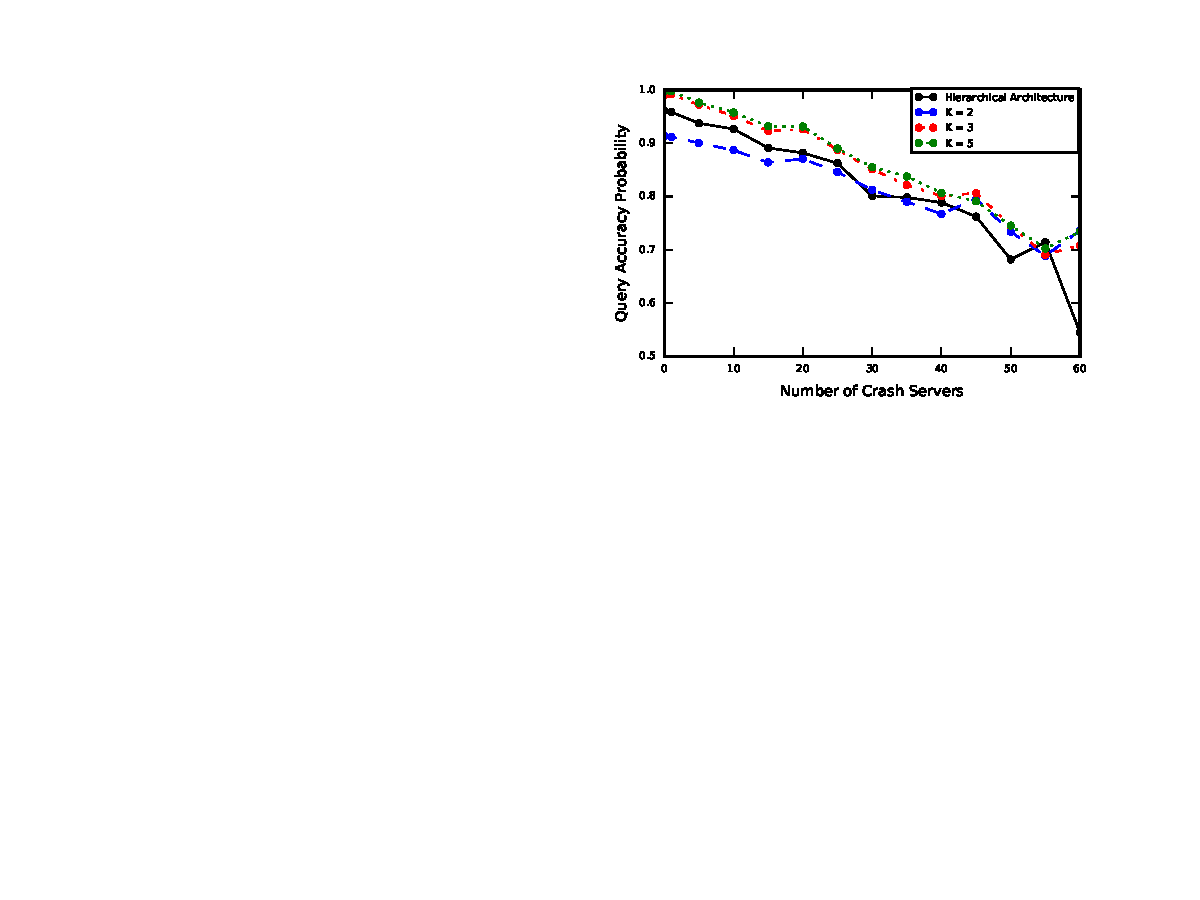
\includegraphics[scale=0.7]{r3} \\
  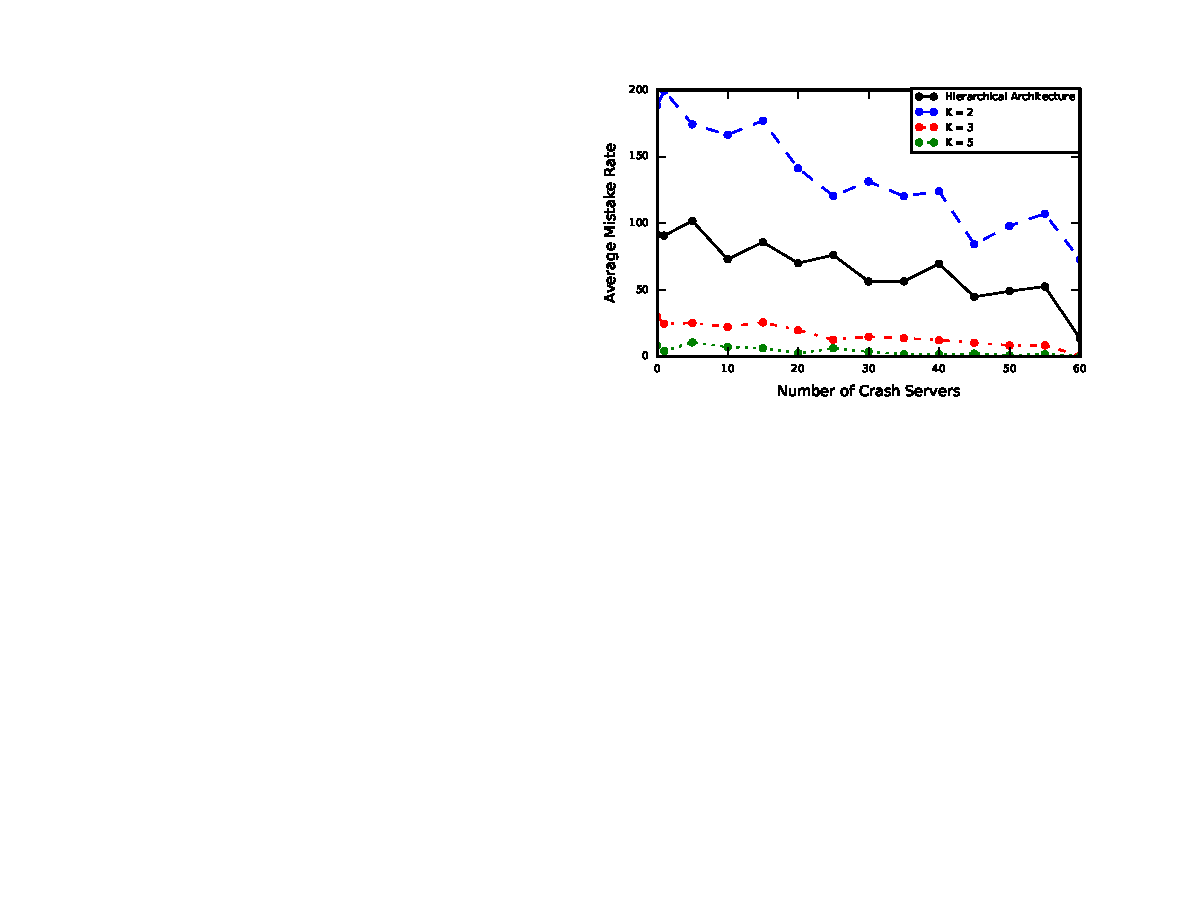
\includegraphics[scale=0.7]{r4} \\
  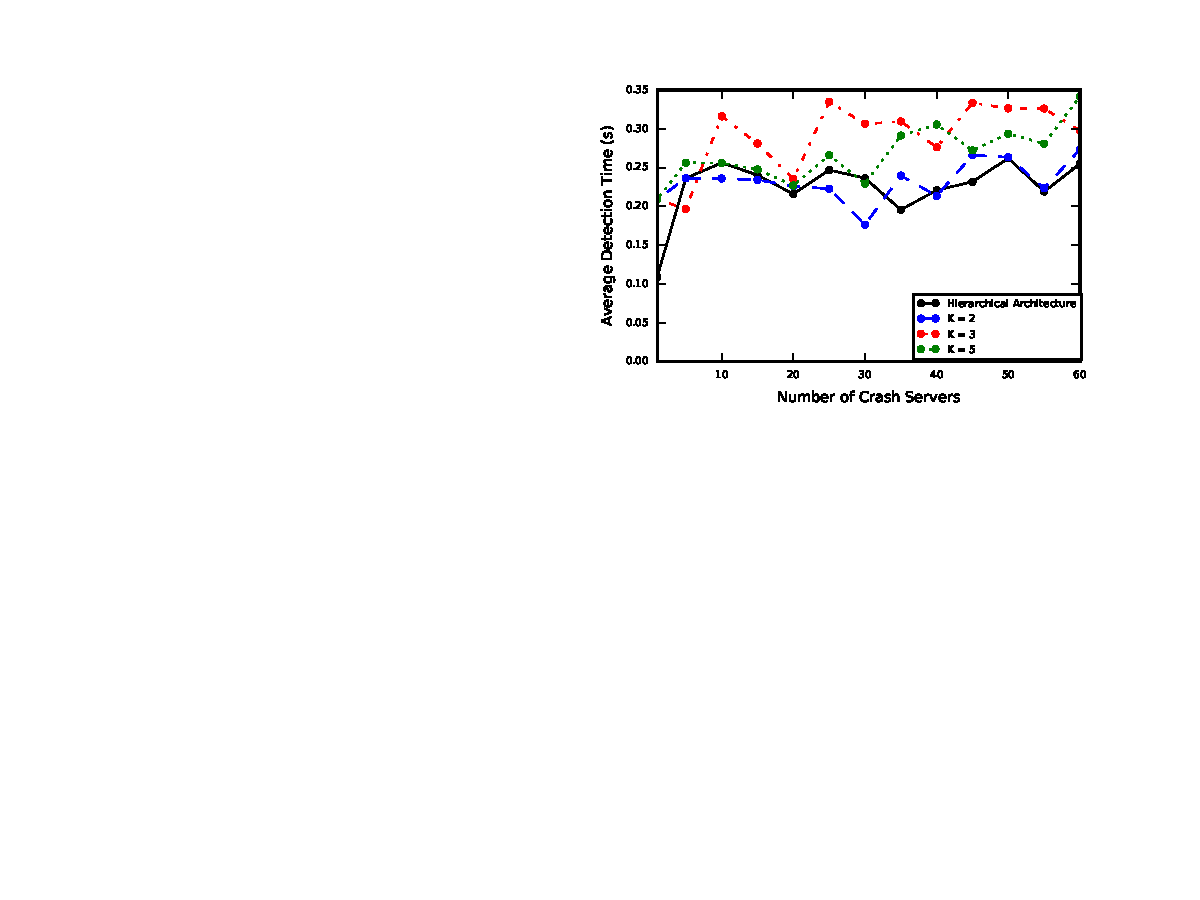
\includegraphics[scale=0.7]{r5} \\
  \end{tabular}
  \caption{Effect of Crashes on $P_A$, $AR_M$ and $AT_D$}
\end{figure}

Figure 5 depicts $P_A$ and $AR_M$ of K-detectors and hierarchical architecture under different number of message loss without server crashes. Both the time and channel of message loss is chosen randomly. When loss rate is under 1\%, 5-detectors has about an 8.2\% improvement in $P_A$ compared with hierarchical architecture. When loss rate is over 0.6\%, 5-detectors makes more mistakes than others, this is probably because other methods make mistakes with relatively longer time. In a nutshell, with a larger parameter $K$, our approach behaves better in the presence of normal message loss. However, it cannot maintain with the increasing number of message loss.

Subsequently, we investigate it when there exists server crashes. We set message loss rate to 0.1\%, both the time and server ID of crashes are selected randomly. As is shown in Figure 6, 5-detectors has a better $P_A$ and $AR_M$ than others in most cases. In terms of $AD_T$, a smaller $K$ results in a quicker detection because it needs fewer FDs to reach an agreement. In general, $AD_T$ of 5-detectors has a 22.4\% increase, while 2-detectors only has a 7.3\% increase compared with hierarchical architecture. Figure 7 shows the number of undetected crashes, hierarchical architecture tends to behave worse than K-detectors, which reveals the \textit{Single Point of Failure} problem of hierarchical architecture.

\begin{figure}[t]
  \centering
  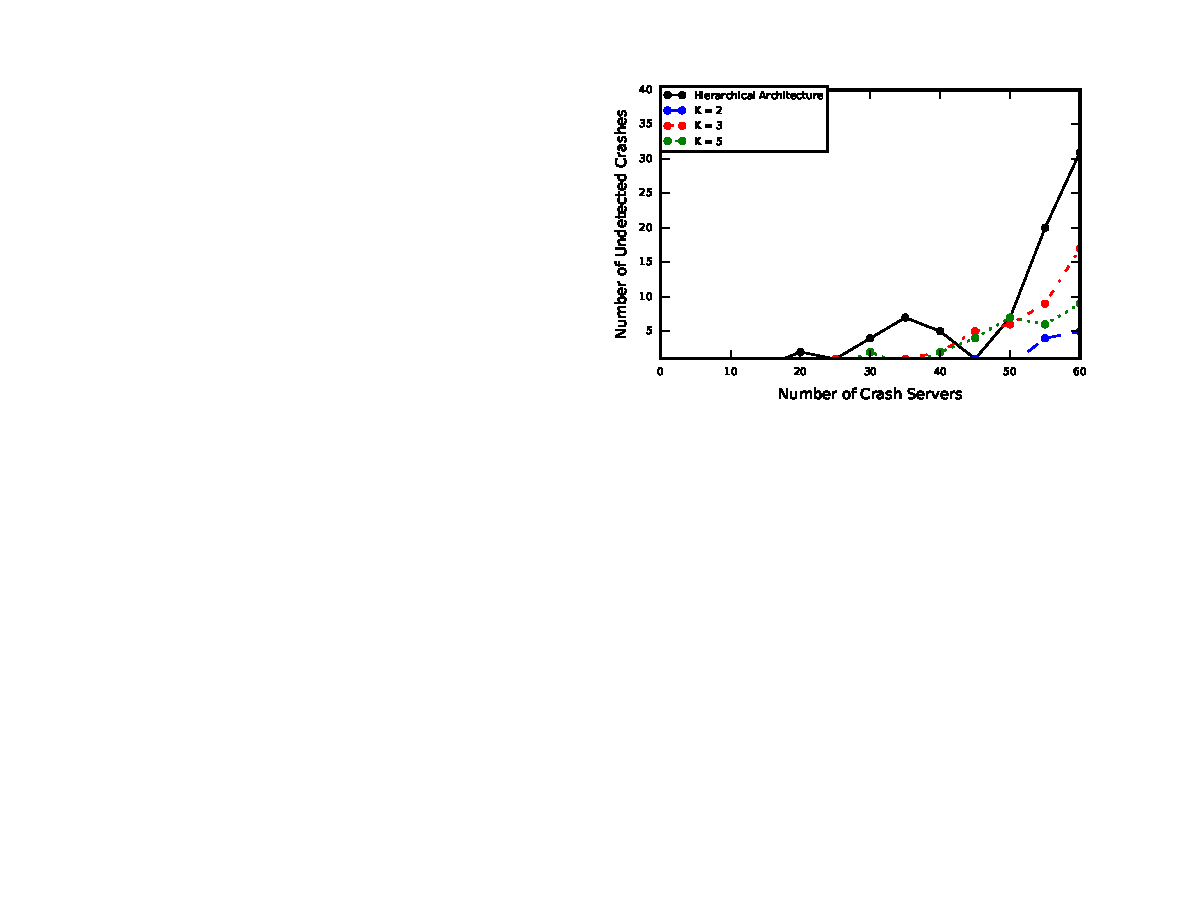
\includegraphics[scale=0.7]{r6}
  \caption{Number of Undetected Crash Servers}
\end{figure}

\subsubsection*{RQ2: ToR failure Detection}
\quad To answer this question, we compute the metrics of ToRs failure detection in the presence of different server crashes. On top of this, we randomly make three ToR failure events with failure group size equals to 1, 2 and 3 respectively. In particular, $\alpha$ is set to 0.9, 0.6 and 0.4 when failure group size is 1, 2 and 3 respectively.

$AR_M$ is all 0 for all the failure events. The $P_A$ and $AD_T$ are shown in Figure 8. Roughly speaking, size of server crashes has little impact on QoS of ToR failure detection. With the increasing of ToR crashes number, $AD_T$ is better due to a smaller $\alpha$, which means \textbf{Crash Decider} needs fewer crash report messages to determine the failure of a ToR.

\begin{figure}[t]
  \centering
  \begin{tabular}{c}
  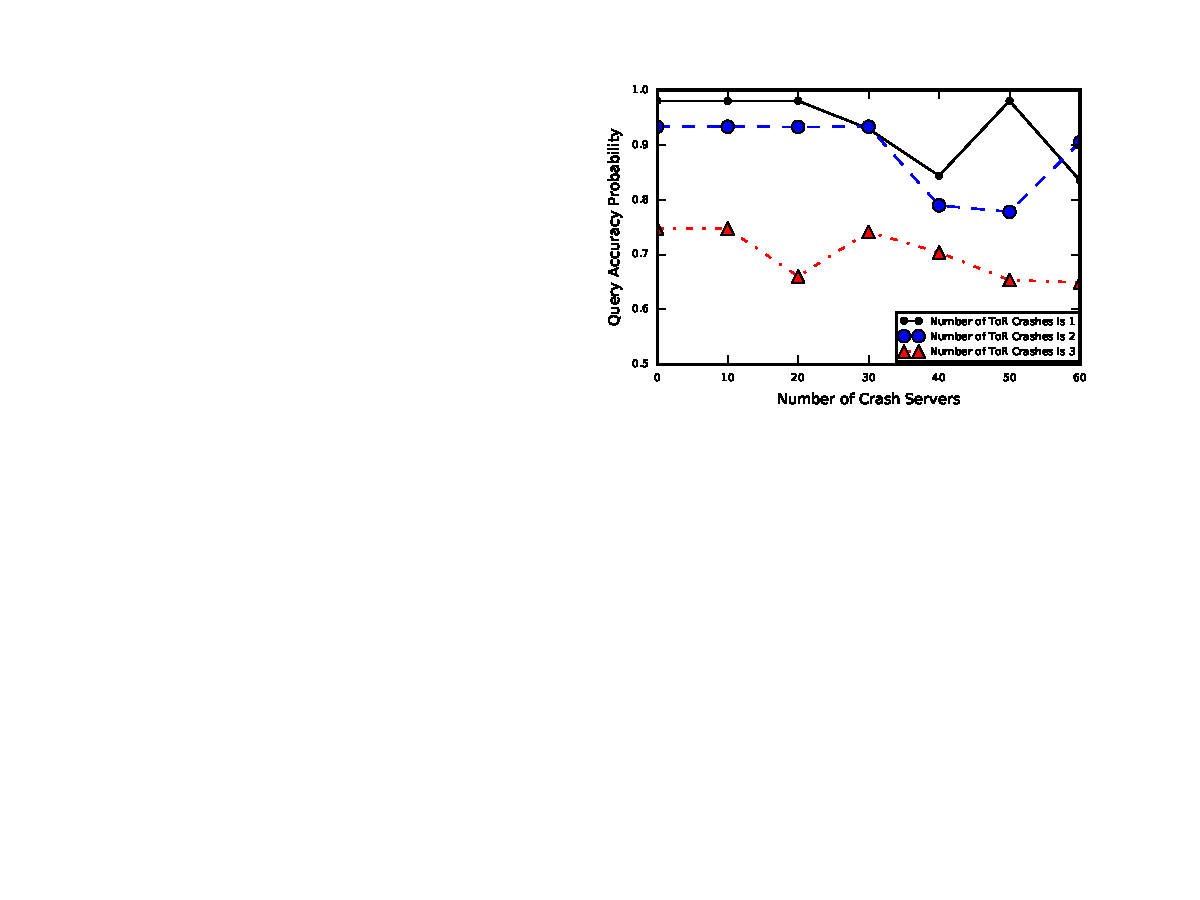
\includegraphics[scale=0.7]{tor-r1} \\
  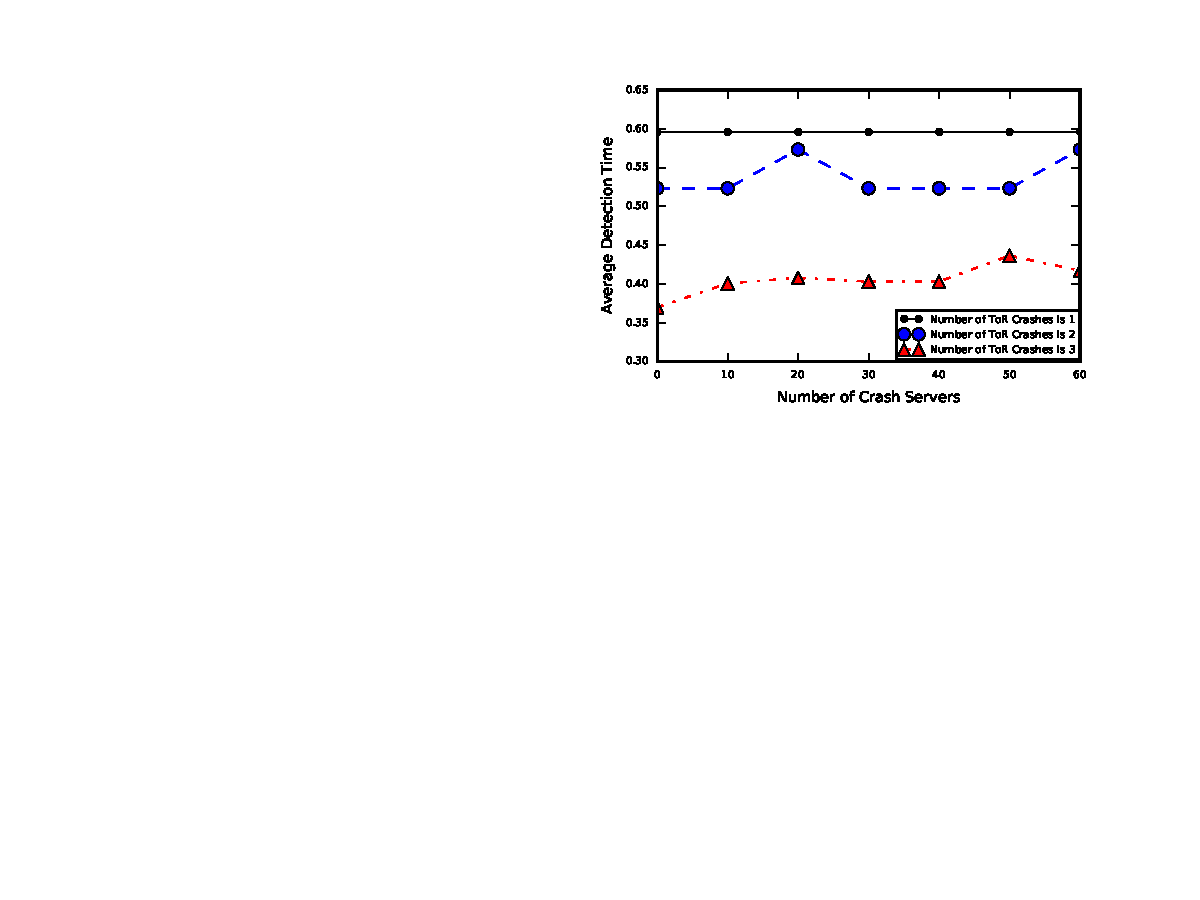
\includegraphics[scale=0.7]{tor-r2} \\
  \end{tabular}
  \caption{Effect of Server Crashes on $P_A$ and $AT_D$ of ToRs}
\end{figure}

The main drawback of our approach is that once occurring ToR failures, we cannot detect server crashes within the rack before the ToR recovers.


\subsubsection*{RQ3: Link failure detection}
\quad To answer this question, we wants to firstly explain why we select BPNN rather other popular classifiers. We select 3 other algorithms including Decision Tree (C4.5) \cite{quinlan2014c4}, Bayesian Networks (BN) \cite{jensen1996introduction} and Support Vector Machine (SVM) \cite{scholkopf1999advances}. We apply these algorithms to train data by 10-fold cross-validation. Results are all shown in Table 1. Obviously BPNN outperforms other algorithms.

\begin{table}
    \centering
    \caption{Results of Different Classifiers}
    \begin{tabular}{|c|c|c|c|} \hline
        \textbf{Classifier} & \textbf{Precision} & \textbf{Recall} & \textbf{F-Measure} \\ \hline
        \hline
        \textbf{BPNN} & 98.8\% & 98.8\% & 98.8\% \\ \hline
        \textbf{C4.5} & 96.4\% & 96.3\% & 96.3\% \\ \hline
        \textbf{BN} & 96.9\% & 96.6\% & 96.7\% \\ \hline
        \textbf{SVM} & 96.9\% & 96.6\% & 96.7\% \\ \hline
    \end{tabular}
\end{table}

\begin{figure}[t]
  \centering
  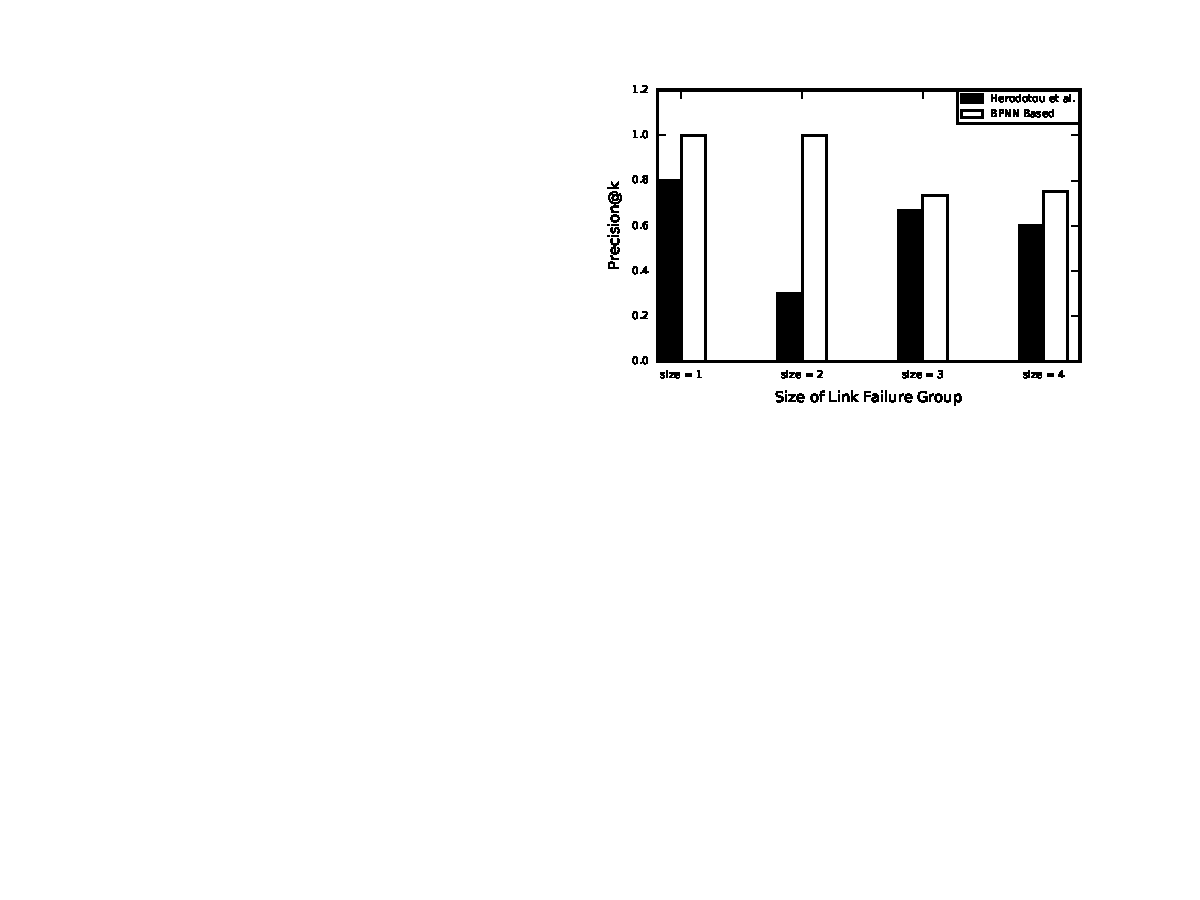
\includegraphics[scale=0.7]{precision} \\
  \caption{Precision@k of Different Failure Group Size}
\end{figure}
\begin{figure}[t]
  \centering
  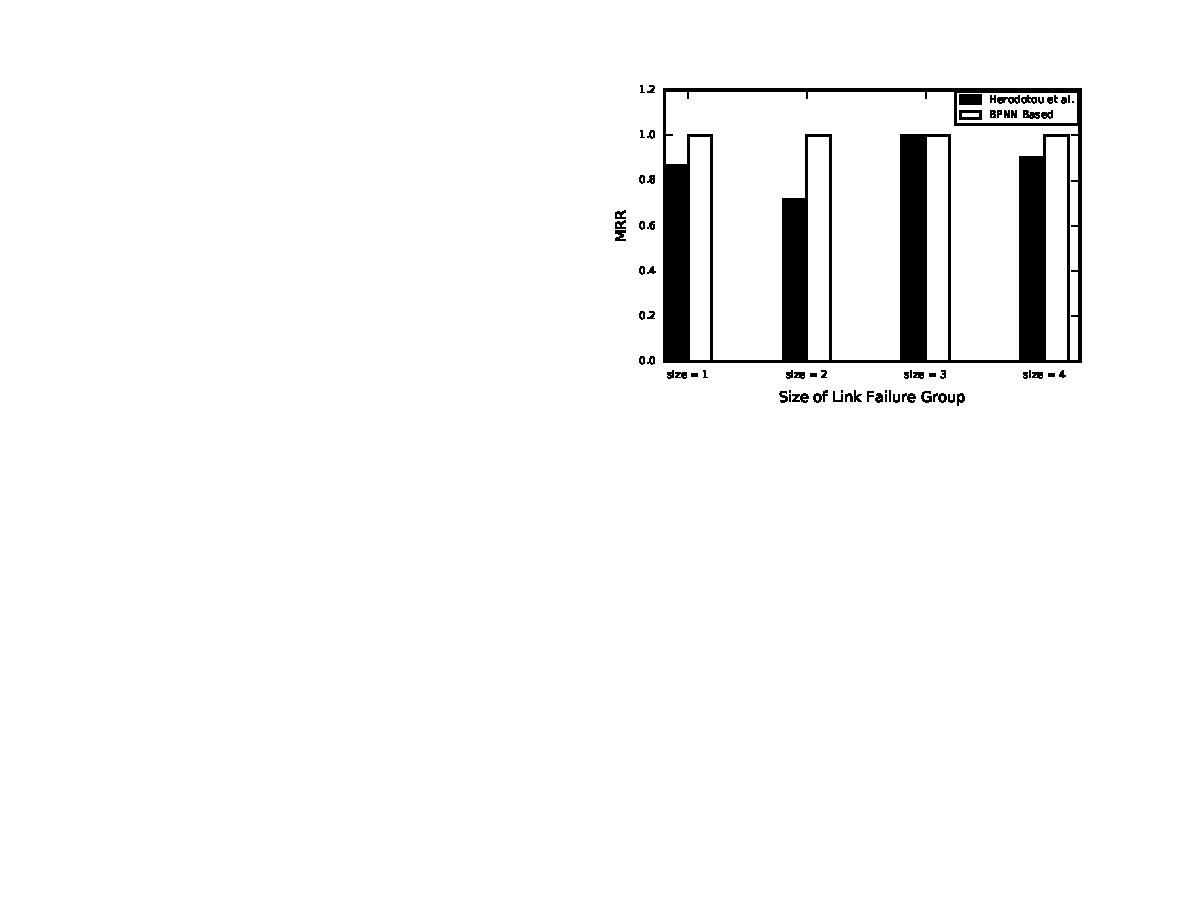
\includegraphics[scale=0.7]{mrr} \\
  \caption{MRR of Different Failure Group Size}
\end{figure}
\begin{figure}[t]
  \centering
  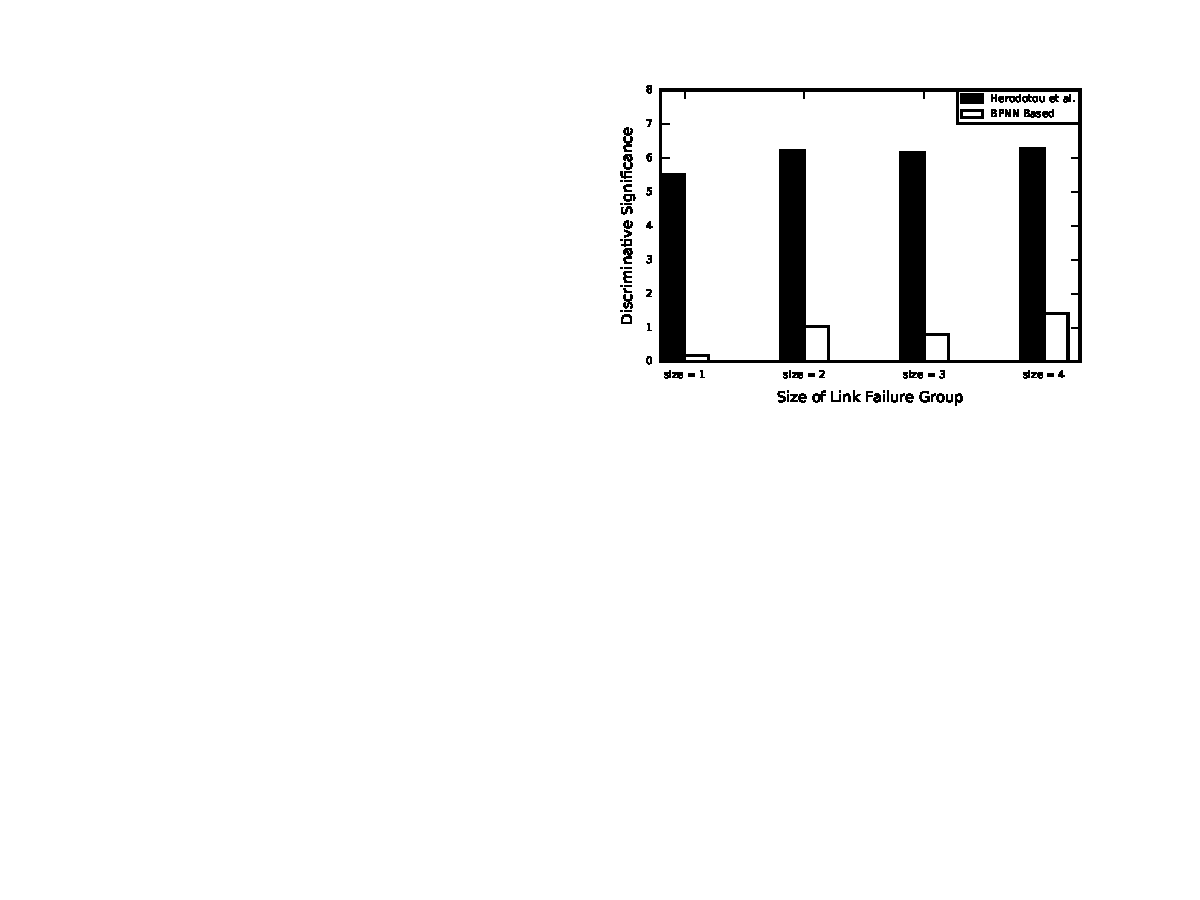
\includegraphics[scale=0.7]{ds} \\
  \caption{DS of Different Failure Group Size}
\end{figure}
Empirically, parameters for BPNN is set as follows: learning rate equals 0.3, number of iterations equals 500, momentum equals 0.2, number of neurons at the hidden layer is $(\# attributes + \# classes) / 2$, $\Delta T = 1 $ s. The selection of $\Delta T$ is a tradeoff, when $\Delta T$ grows bigger, it may contain multiple failures which violates our assumption, while a smaller $\Delta T$ may add more occasionality to traffic data.

We manually make some link failures by disabling links in ns-3, we make 5 random failure events for different size of failure group respectively. Both the link ID and failure time are selected randomly. As Gill et al. finds that link failures tend to be isolated \cite{gill2011understanding}. Only 41\% of the link failure groups contain more than one faults, only 10\% contain more than four faults. Consequently we only make failure events whose failure group size is no more than four.

Figure 9, 10 and 11 show the results of out experiments. Our approach has a better performance in terms of percision@k and MRR. In particular, there is an at least 73.3\% precision@k performance, which indicates 73.3\% of the failures can be found at the most top of the suspects averagely.

On the other hand, there is a huge improvement (nearly 12-folds improvement) in terms of DS. The approach proposed by Herodotou et al. tends to assign a wider range of failure scores to multiple links, while our approach is better at finding the relevant links. It mainly stems from the fact that our approach is based on a multi-layer perceptron architecture, it can precisely capture the characteristic of each link failure. But one of the drawbacks of our approach is that it requires much data and time to train BPNN offline to ensure its generalization ability, it cannot adapt to network topology changes either.



\section{Conclusions}
Failure detection plays a very important role in maintaining the reliability of data center networks. In this paper, we firstly identify the differences in QoS of failure detection for different network devices. We leverage K-detectors model to enhance the timeliness, accuracy and soundness of failure detection for imperative devices. We leverage a data mining based approach to produce a ranked list of the most suspect non-imperative devices by capturing network traffic features. We have implemented our approach as well as baselines on a simulated data center network built by ns-3. Our experimental evaluation has validated the effectiveness of our approach.


\section{Acknowledgments}
This work is partially supported by the National High-Technology Research and Development Program of China under Grant No.2014AA01A301.


\bibliographystyle{abbrv}
\bibliography{paper}

\end{document}








